\chapter{Nuisance Parameter Impact}

The observed and expected ($\mu_{exp}=$0) impacts of the nuisance parameters on the profile likelihood fit are shown in Figure \ref{fig:Impact0}-\ref{fig:Impact1}. They were computed using the following commands and plotted below for full run 2.

 \begin{figure}[tbh!]
 \begin{center}
 \begin{tabular}{cc}
 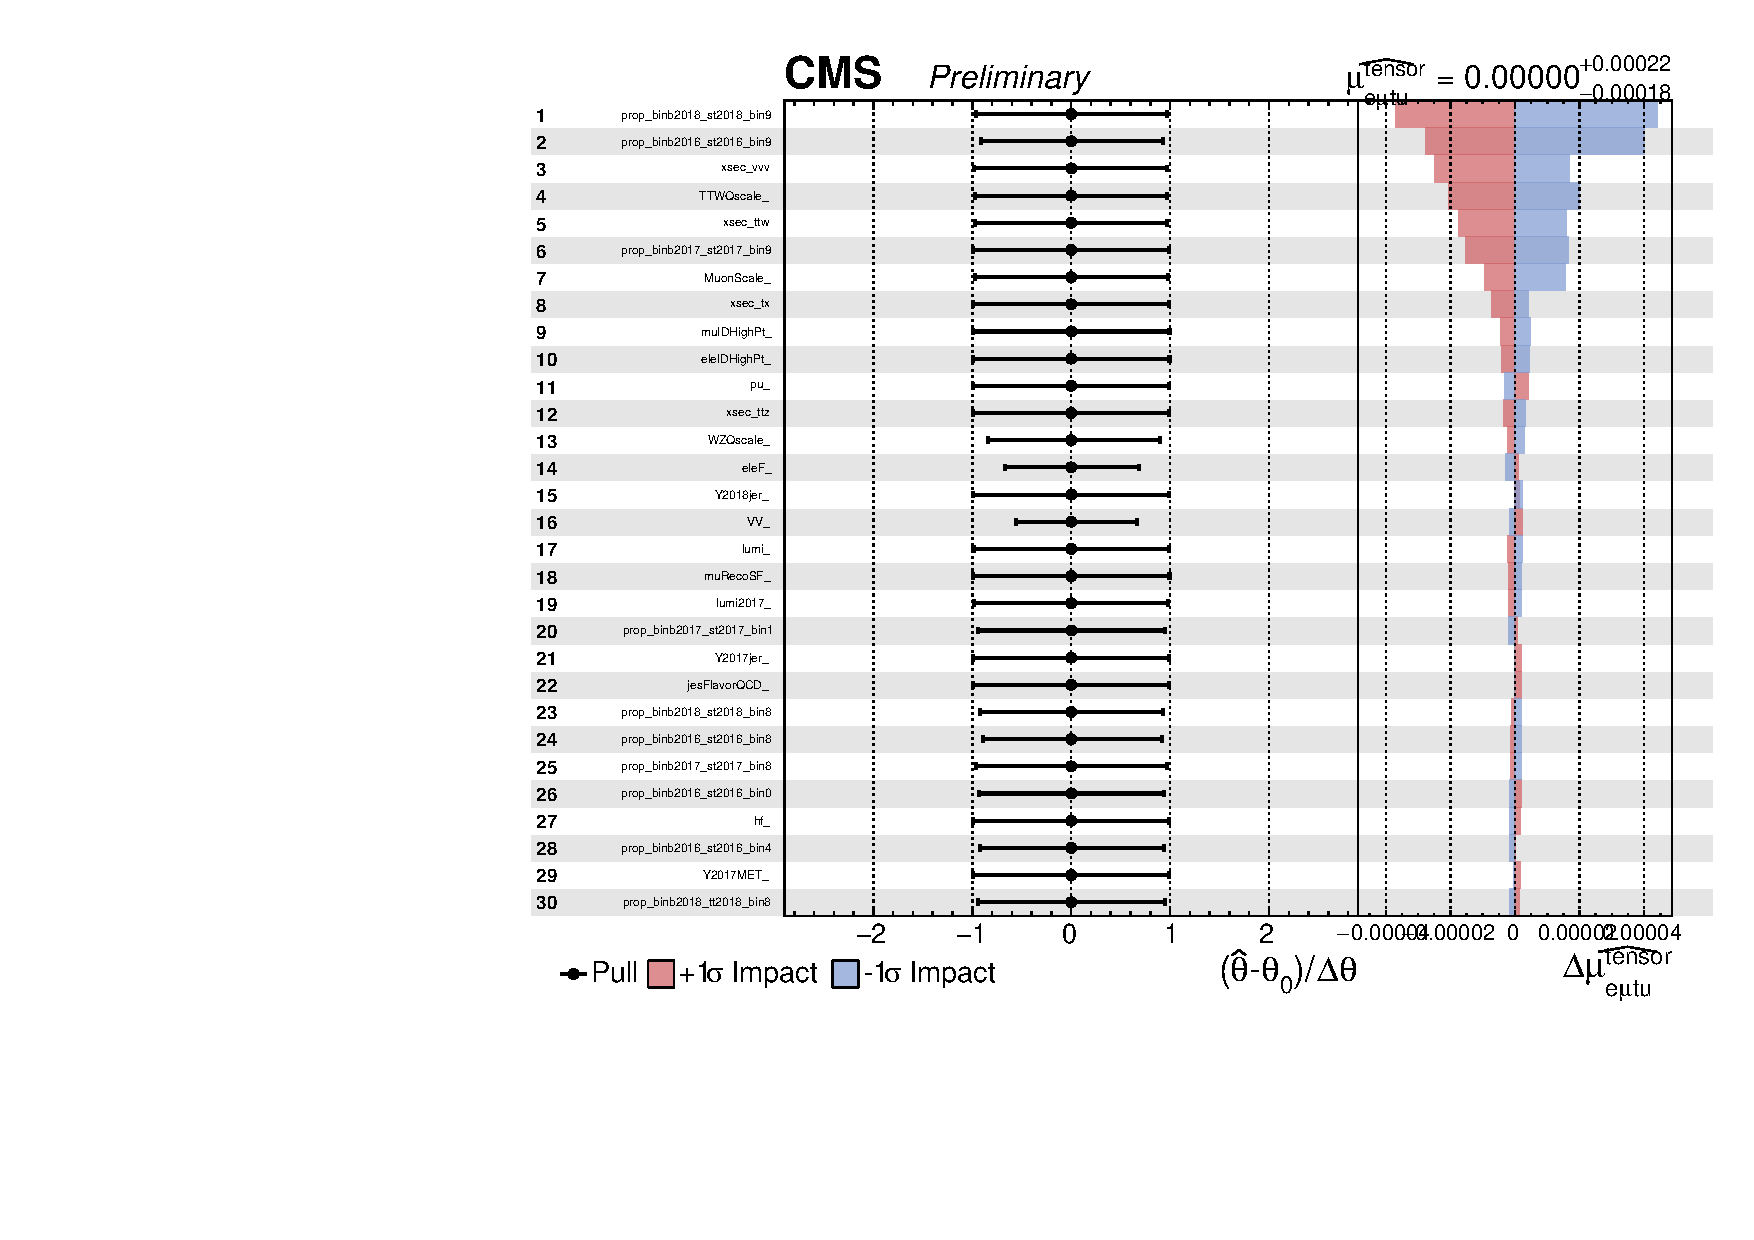
\includegraphics[width=0.48\textwidth]{figures/Appendix/Impact/Impact_TensorU_expected0}&
  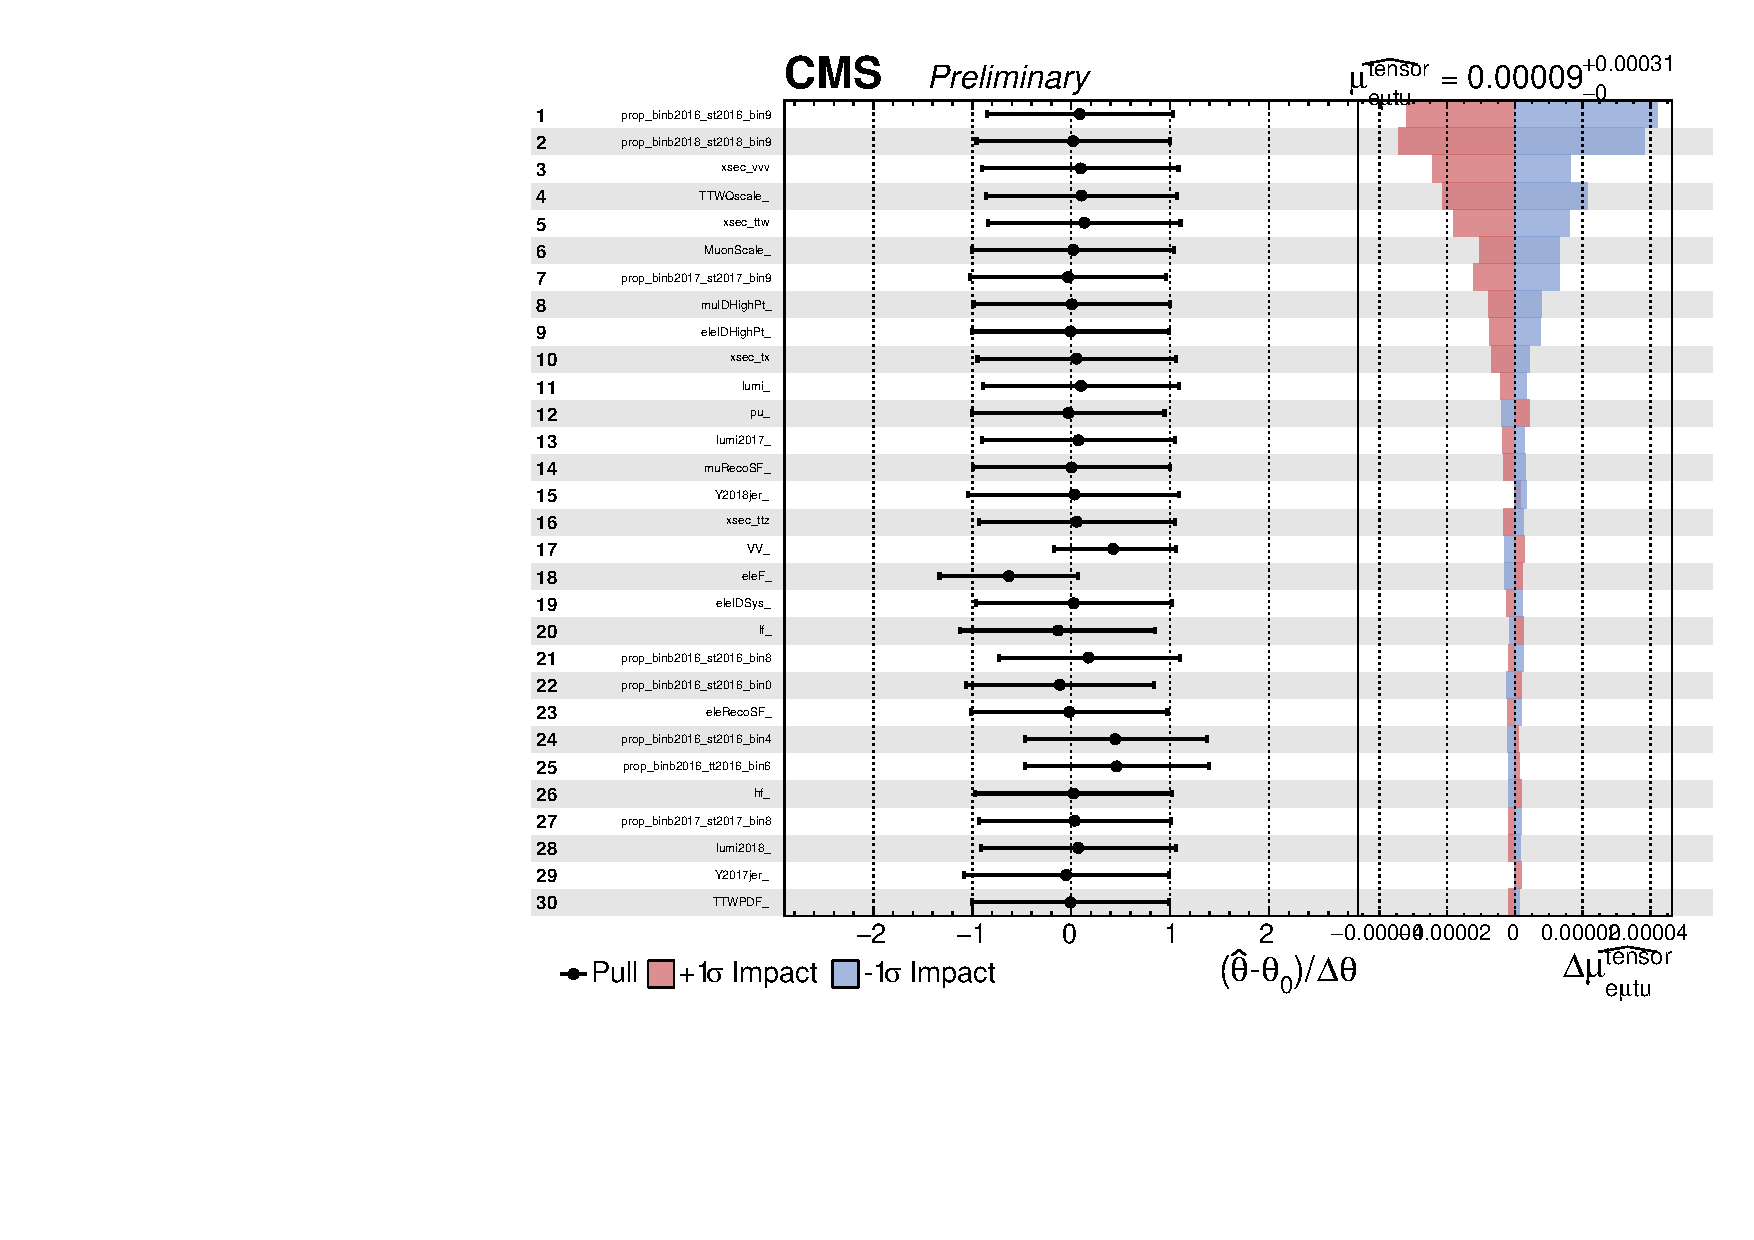
\includegraphics[width=0.48\textwidth]{figures/Appendix/Impact/Impact_TensorU}\\
   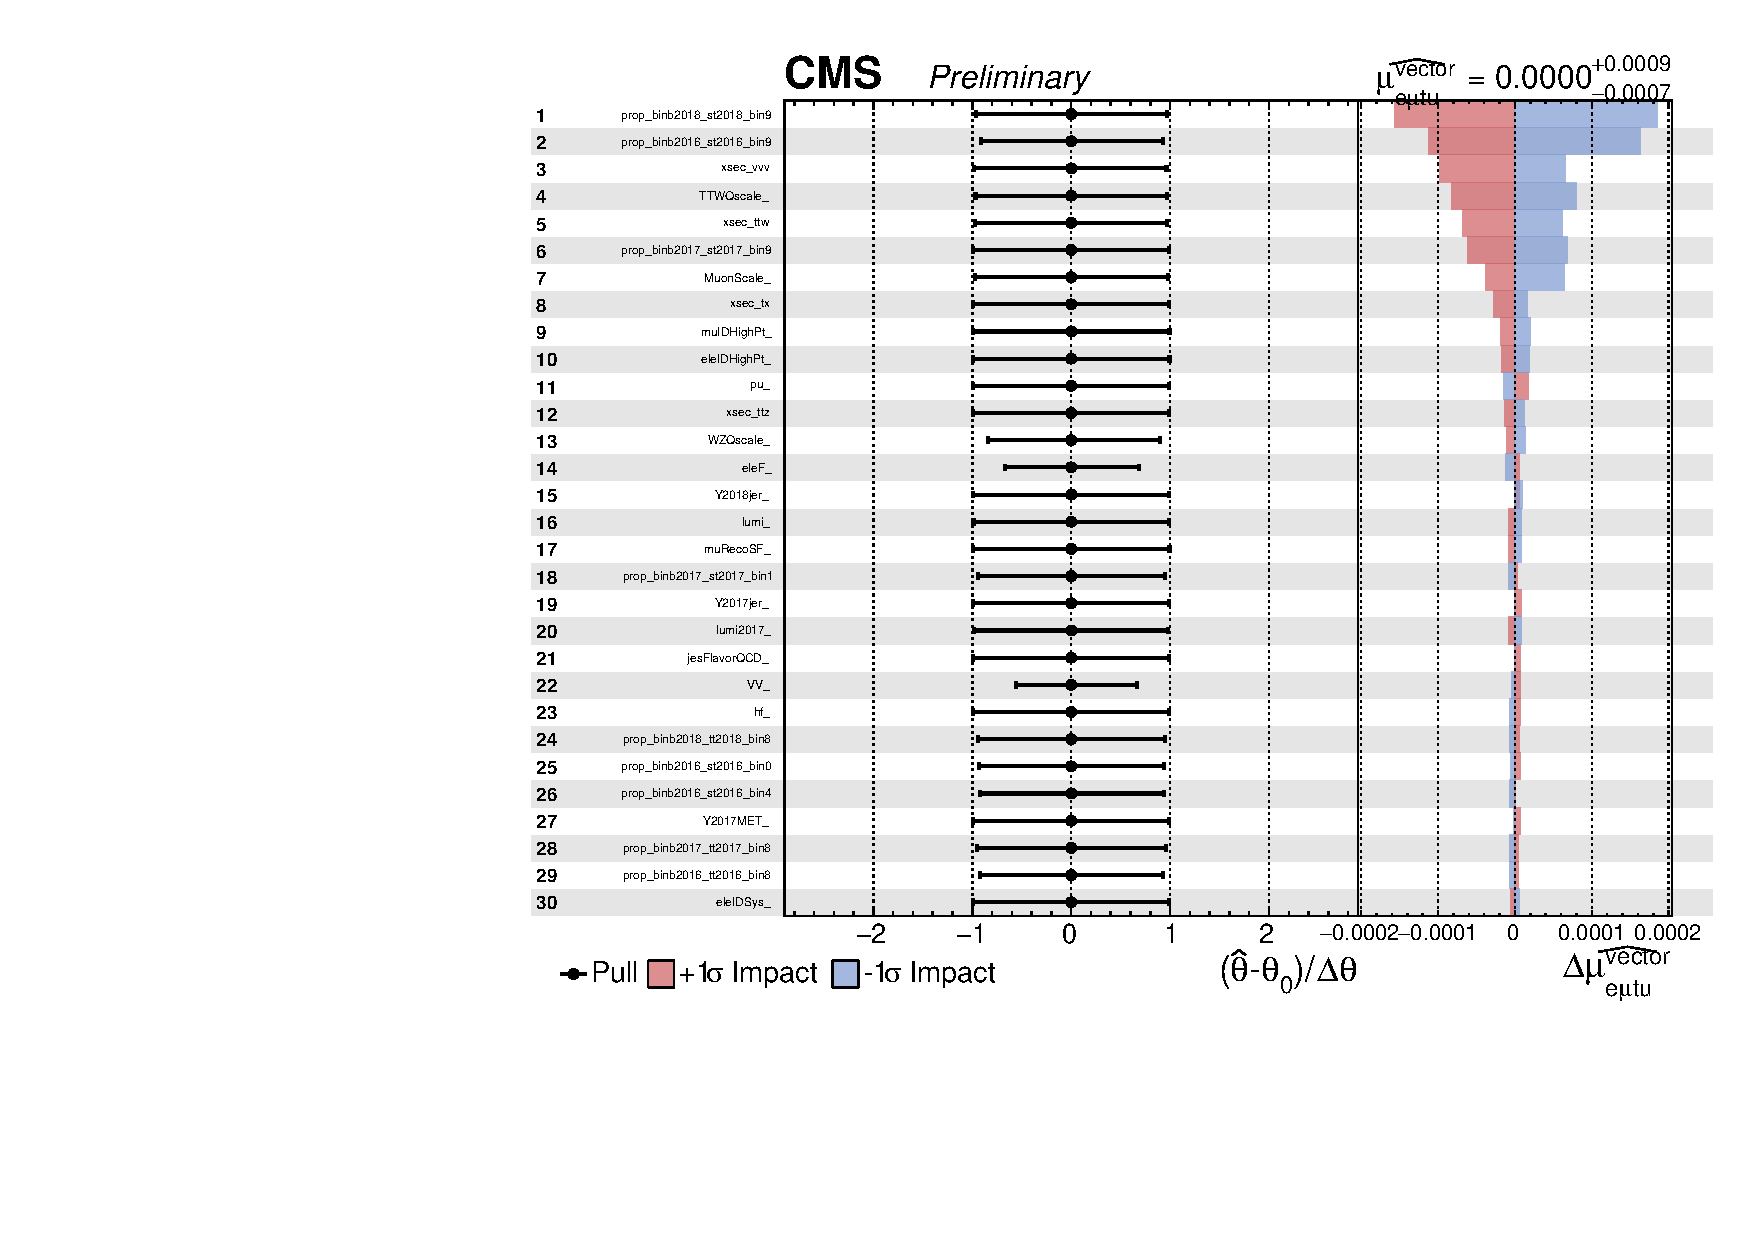
\includegraphics[width=0.48\textwidth]{figures/Appendix/Impact/Impact_VecU_expected0}&
  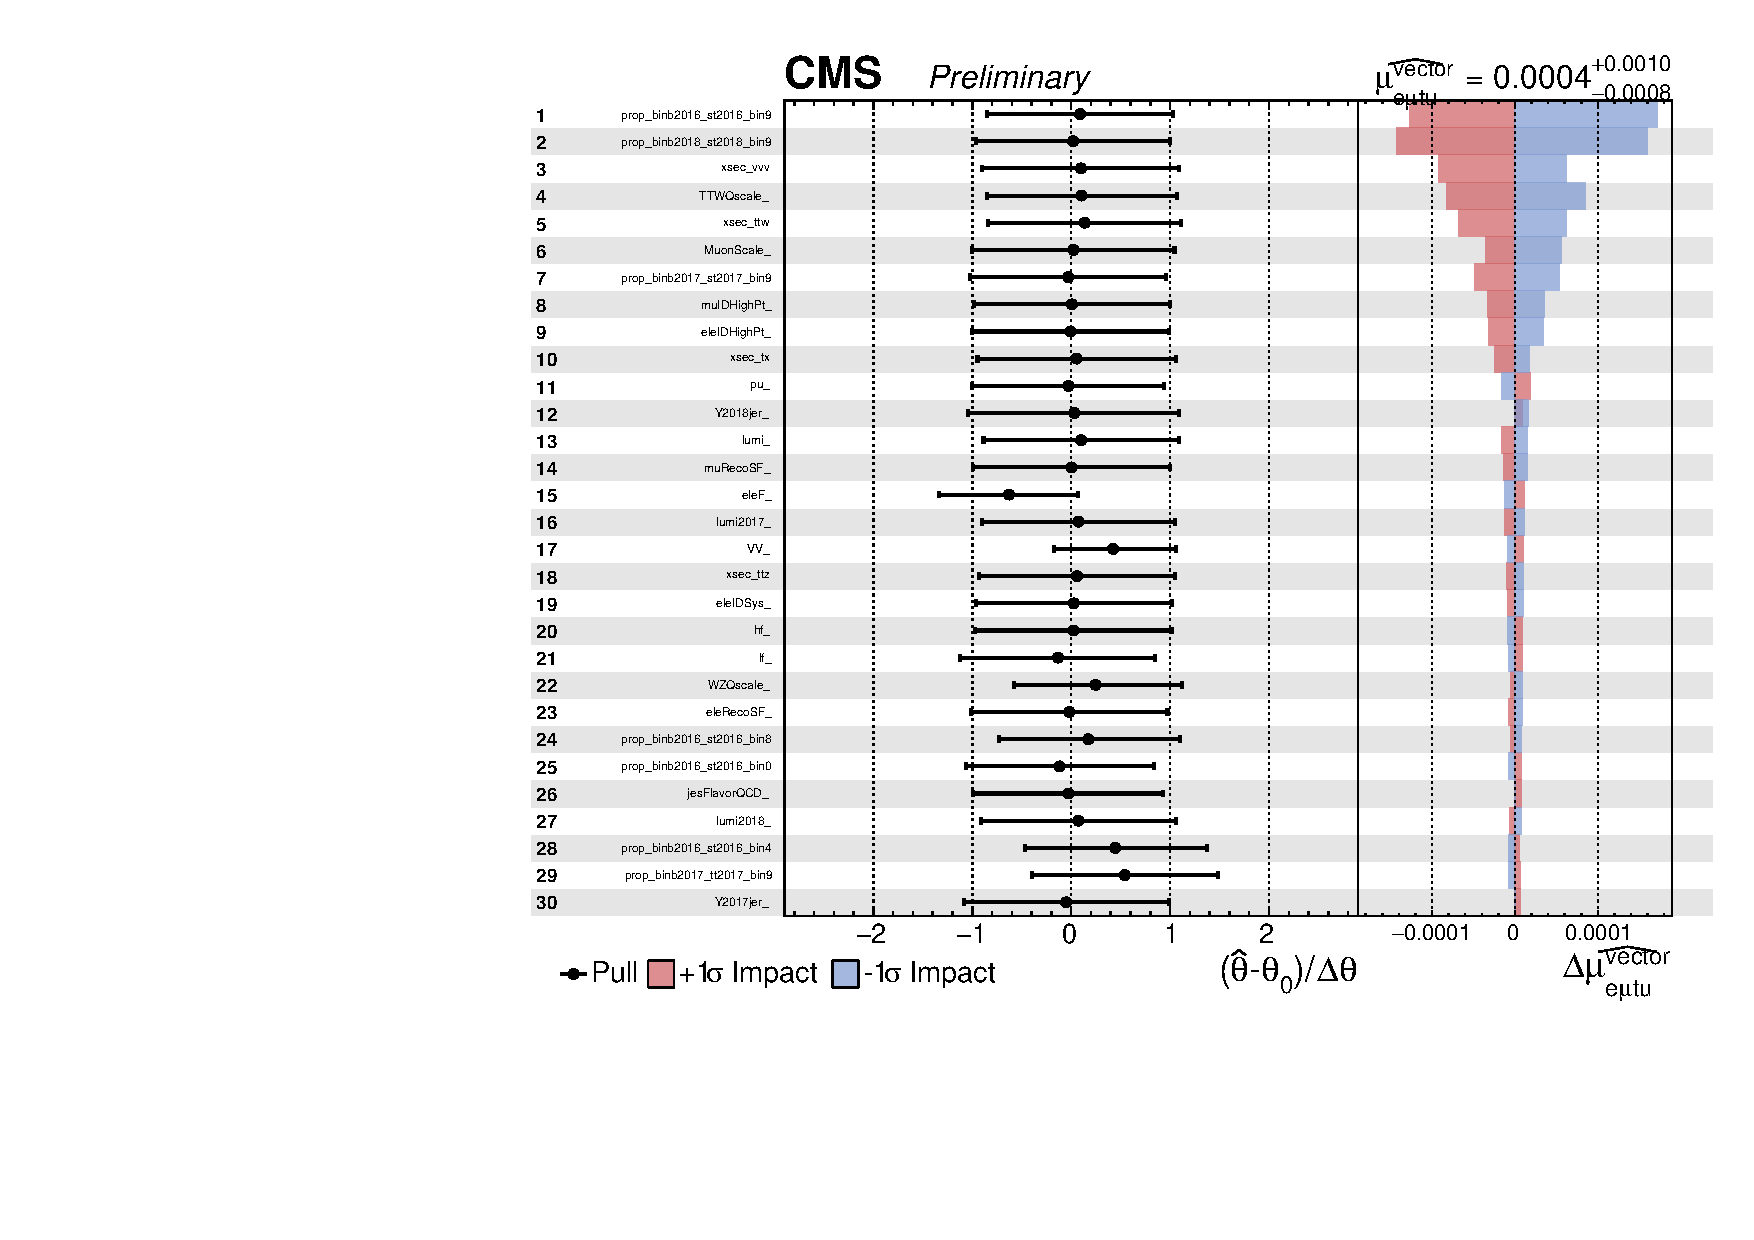
\includegraphics[width=0.48\textwidth]{figures/Appendix/Impact/Impact_VecU}\\
   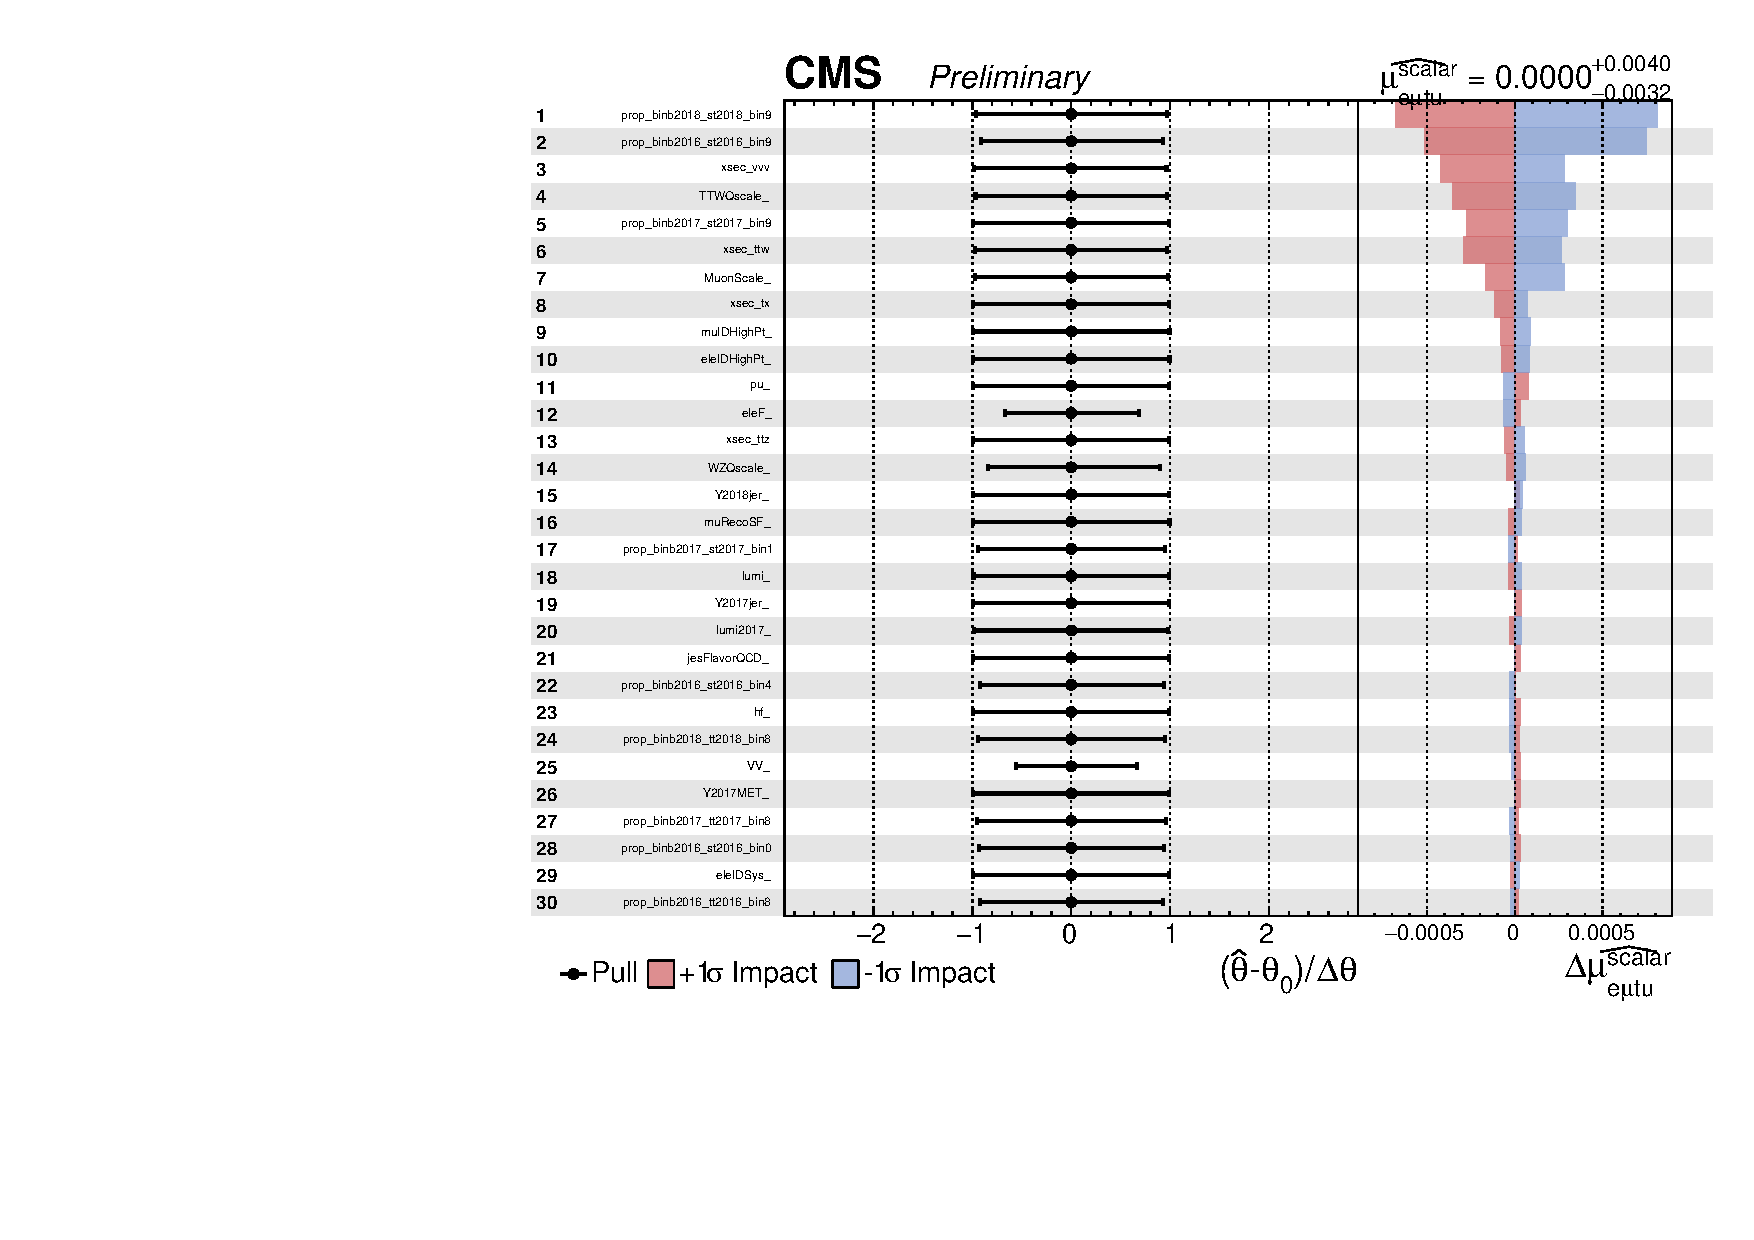
\includegraphics[width=0.48\textwidth]{figures/Appendix/Impact/Impact_ScalarU_expected0}&
  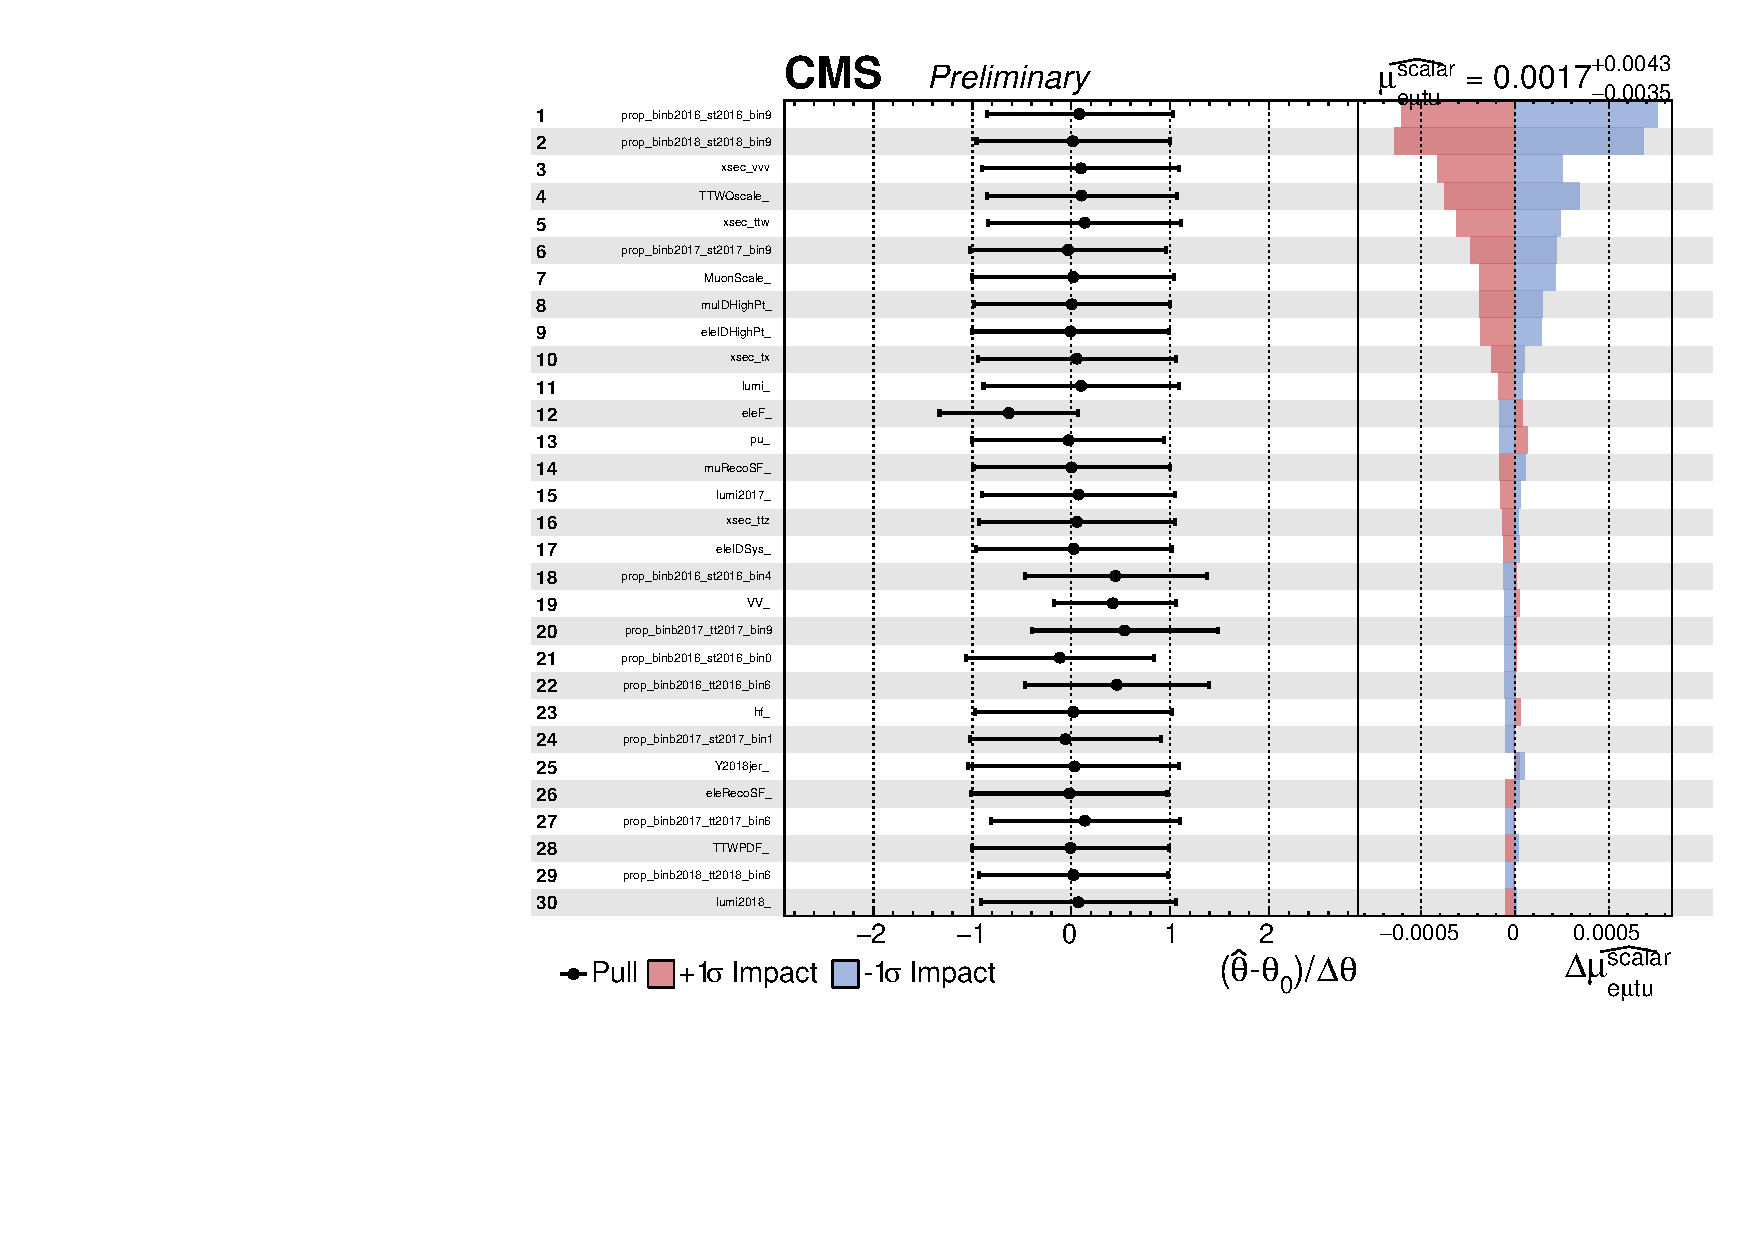
\includegraphics[width=0.48\textwidth]{figures/Appendix/Impact/Impact_ScalarU}\\
 \end{tabular}
 \caption{Impacts of nuissance parameters for run II limit setting. From top to bottom: $e\mu tu$-tensor, $e\mu tu$-vector, $e\mu tu$-scalar. From left to right: expected impact (expected signal strength at 0), observed impact.}
 \label{fig:Impact0}
 \end{center}
\end{figure}

 \begin{figure}[tbh!]
 \begin{center}
 \begin{tabular}{cc}
 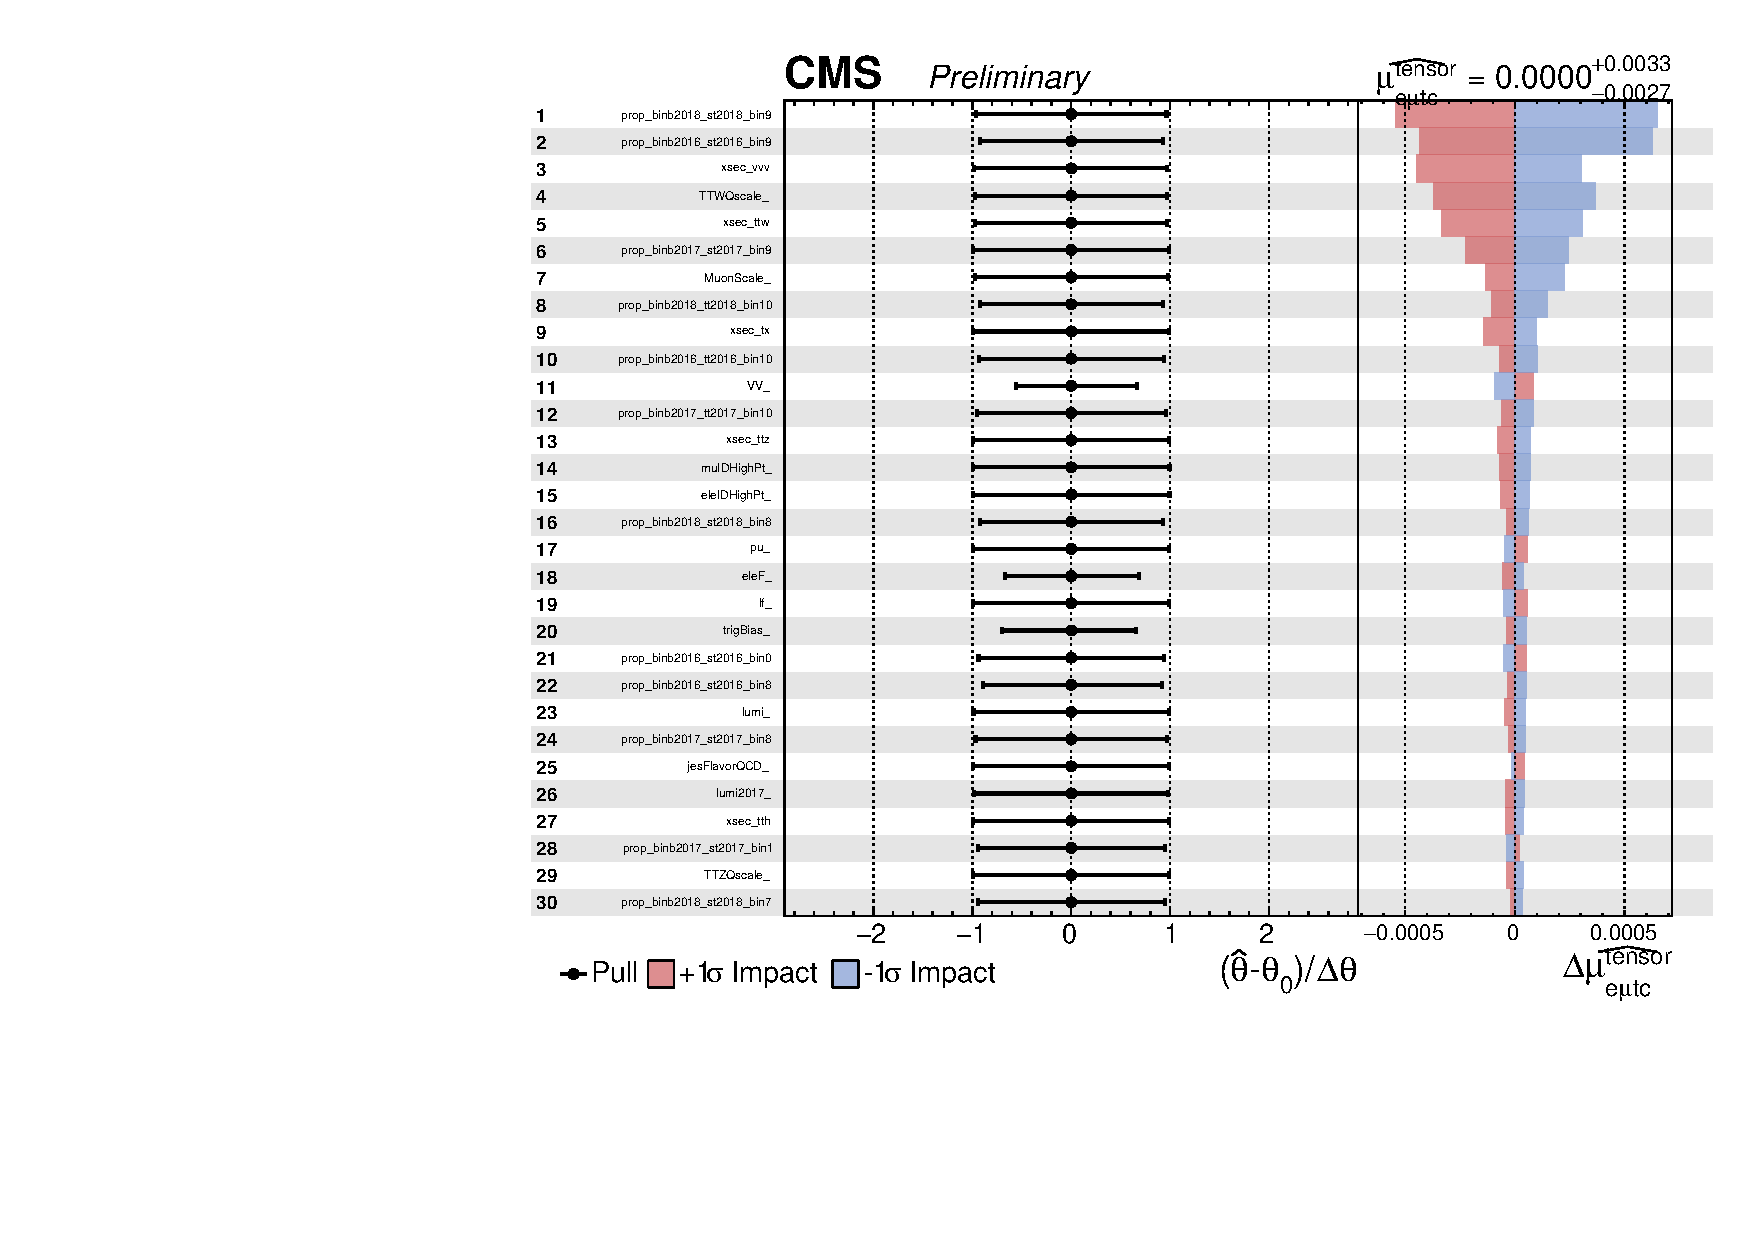
\includegraphics[width=0.48\textwidth]{figures/Appendix/Impact/Impact_TensorC_expected0}&
  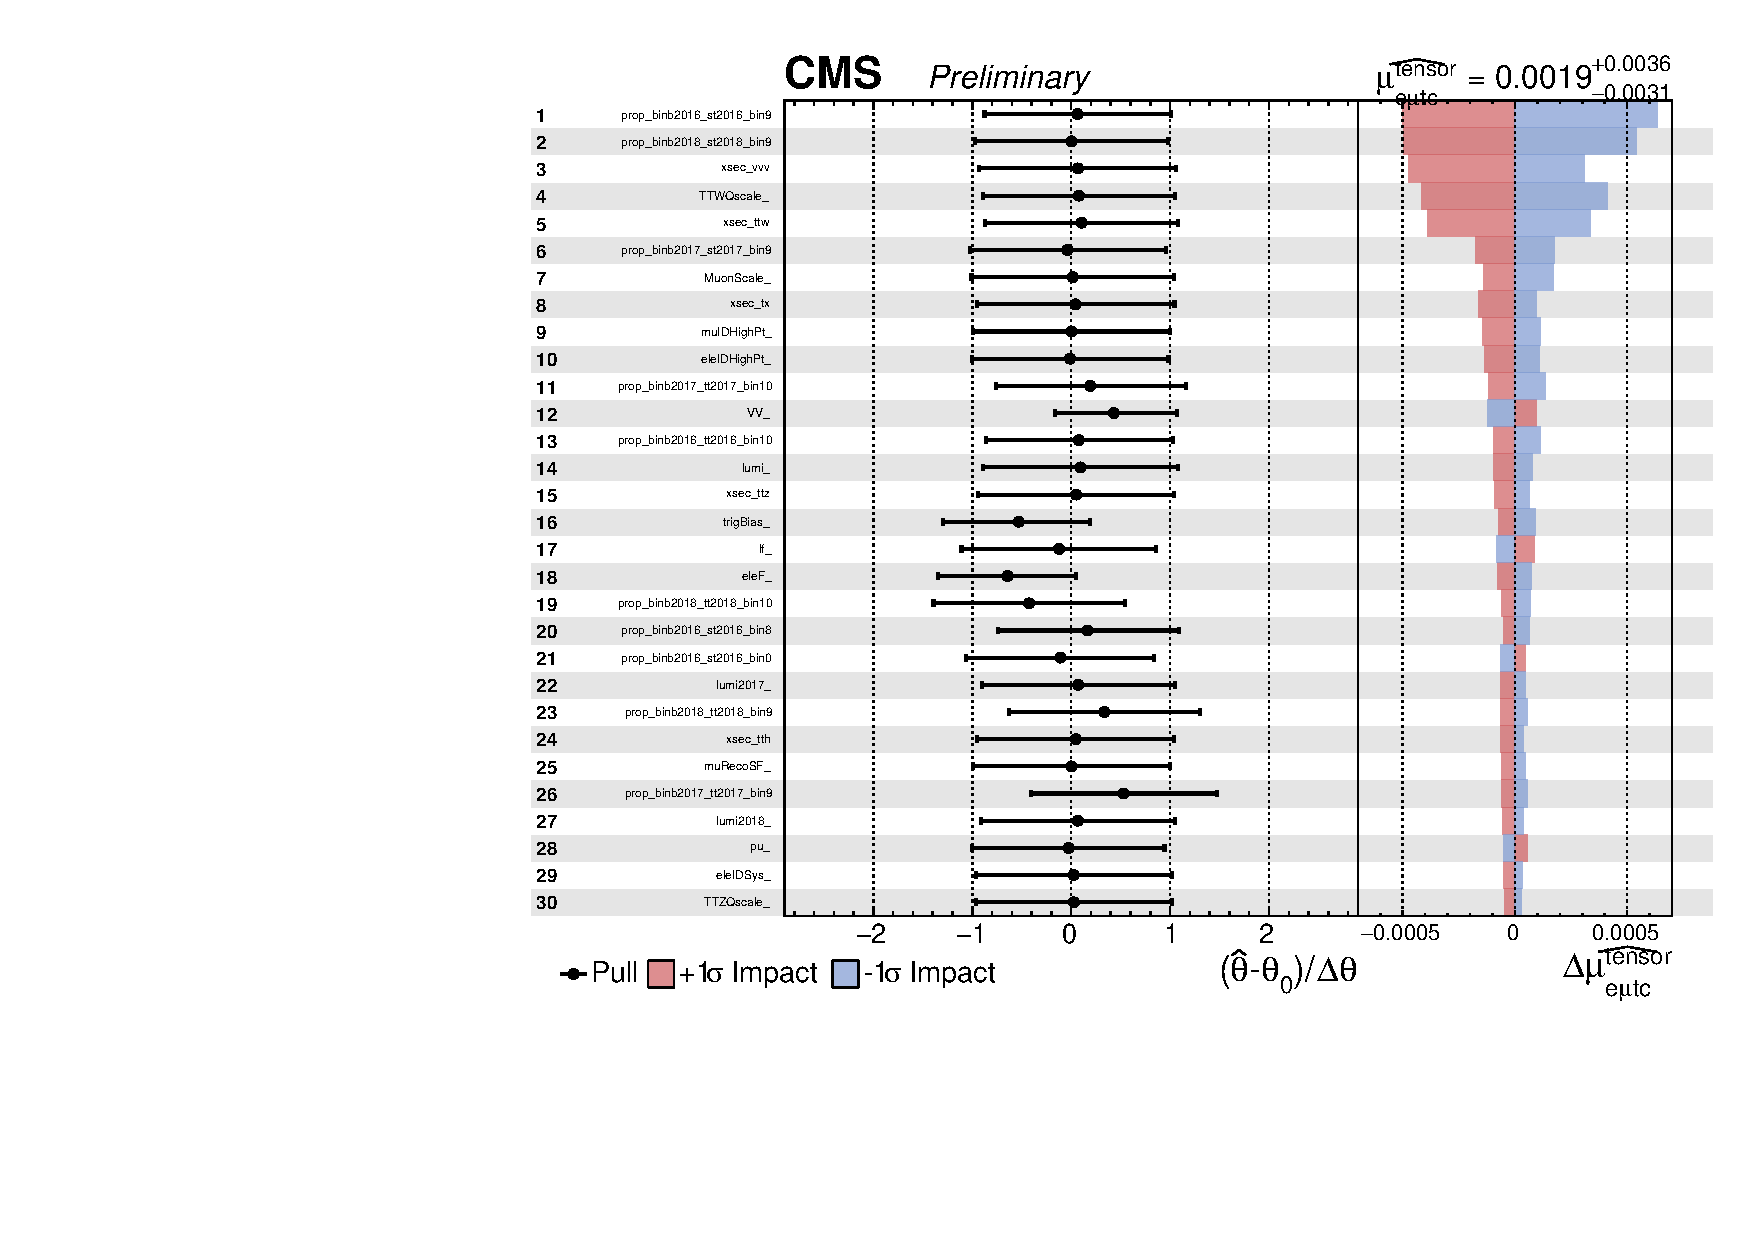
\includegraphics[width=0.48\textwidth]{figures/Appendix/Impact/Impact_TensorC}\\
   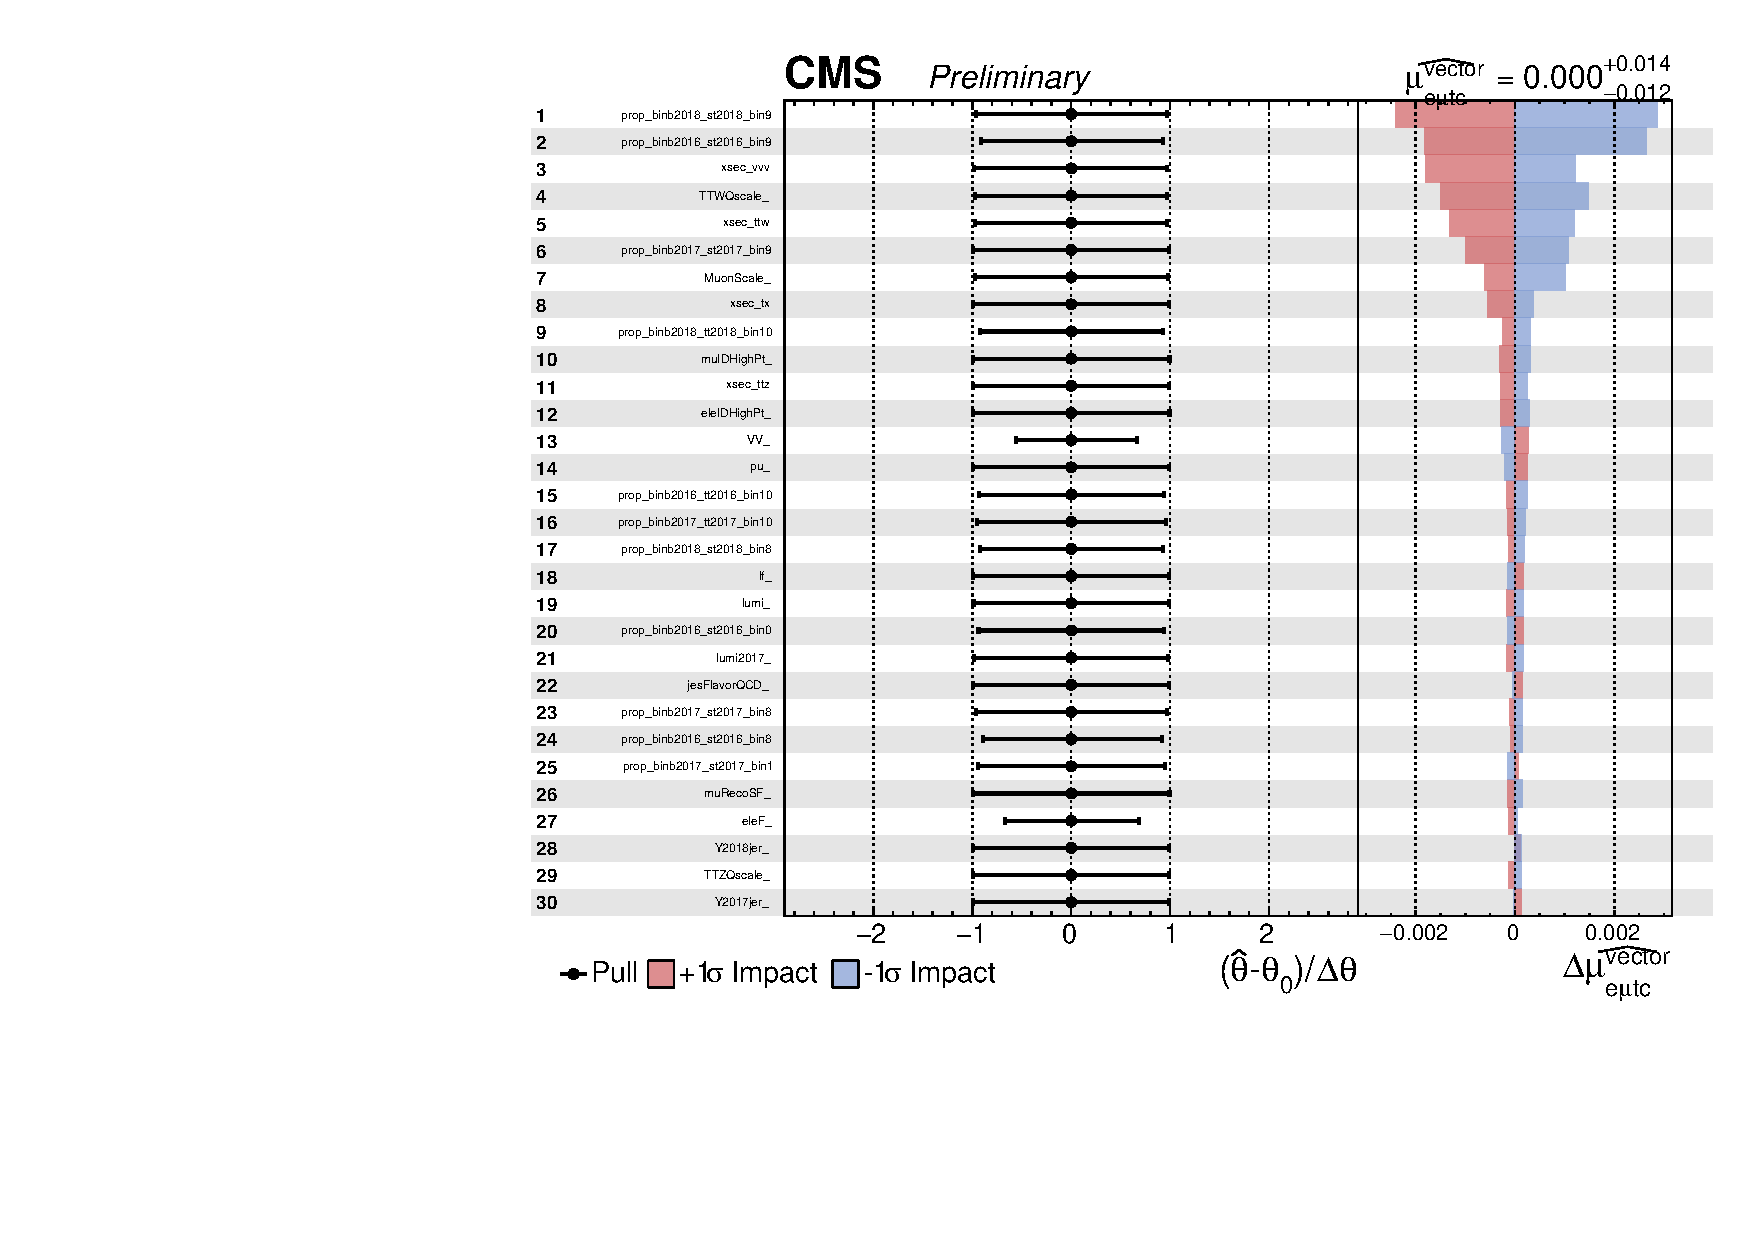
\includegraphics[width=0.48\textwidth]{figures/Appendix/Impact/Impact_VecC_expected0}&
  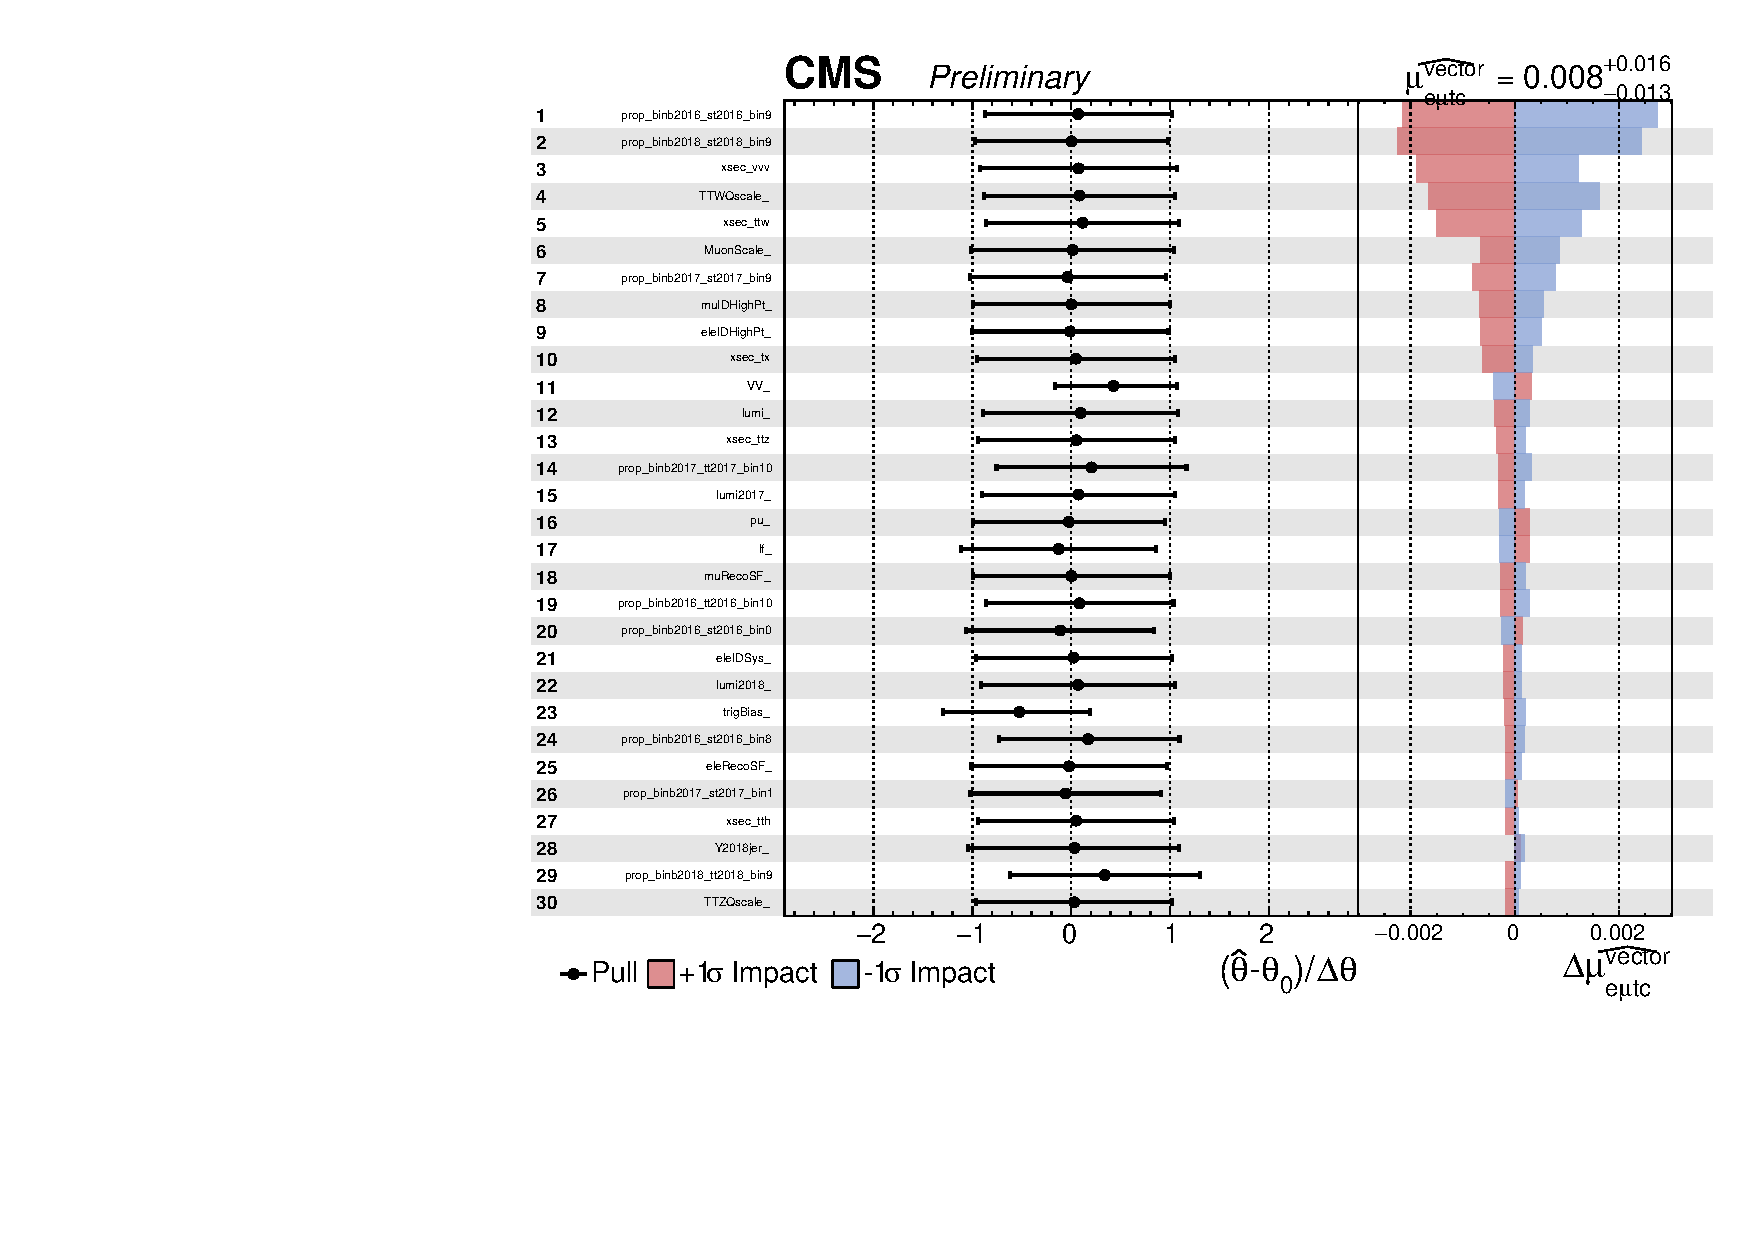
\includegraphics[width=0.48\textwidth]{figures/Appendix/Impact/Impact_VecC}\\
   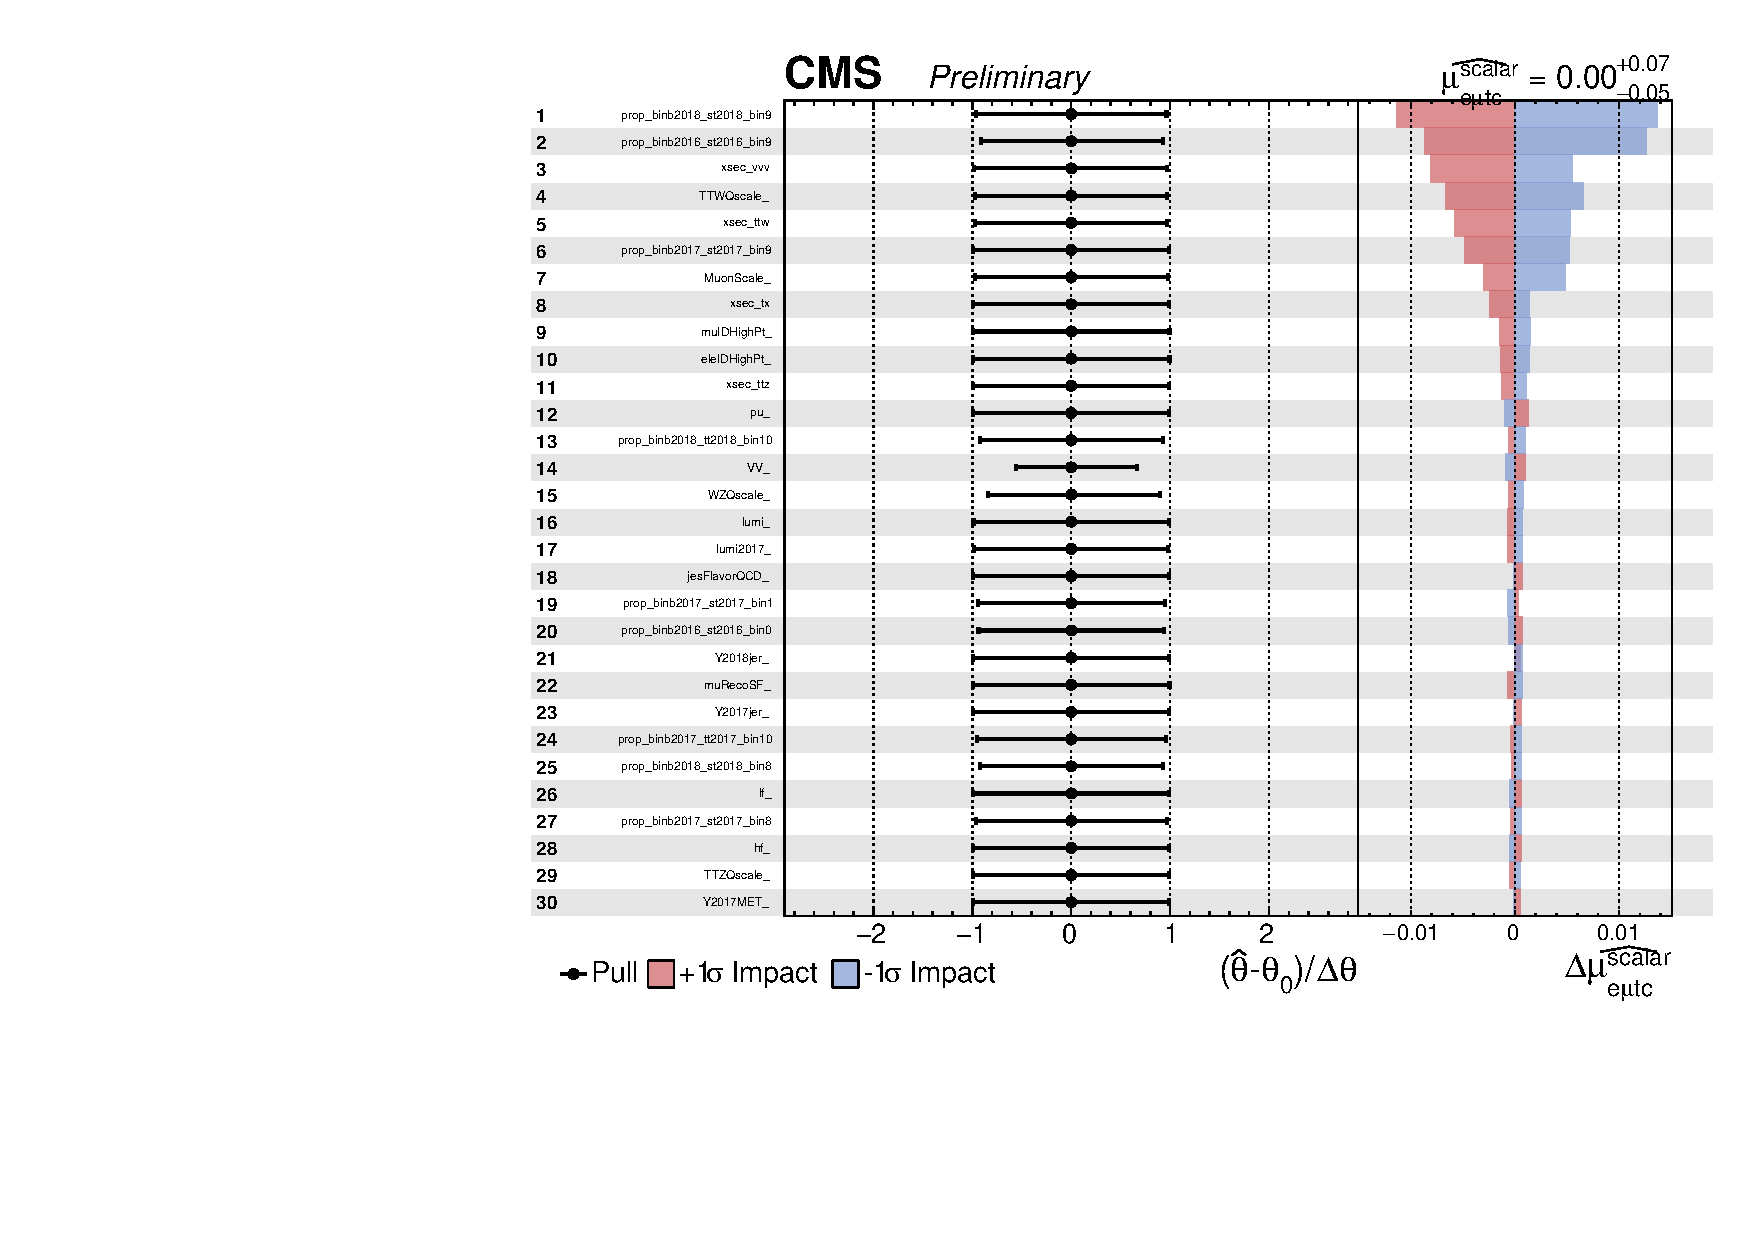
\includegraphics[width=0.48\textwidth]{figures/Appendix/Impact/Impact_ScalarC_expected0}&
  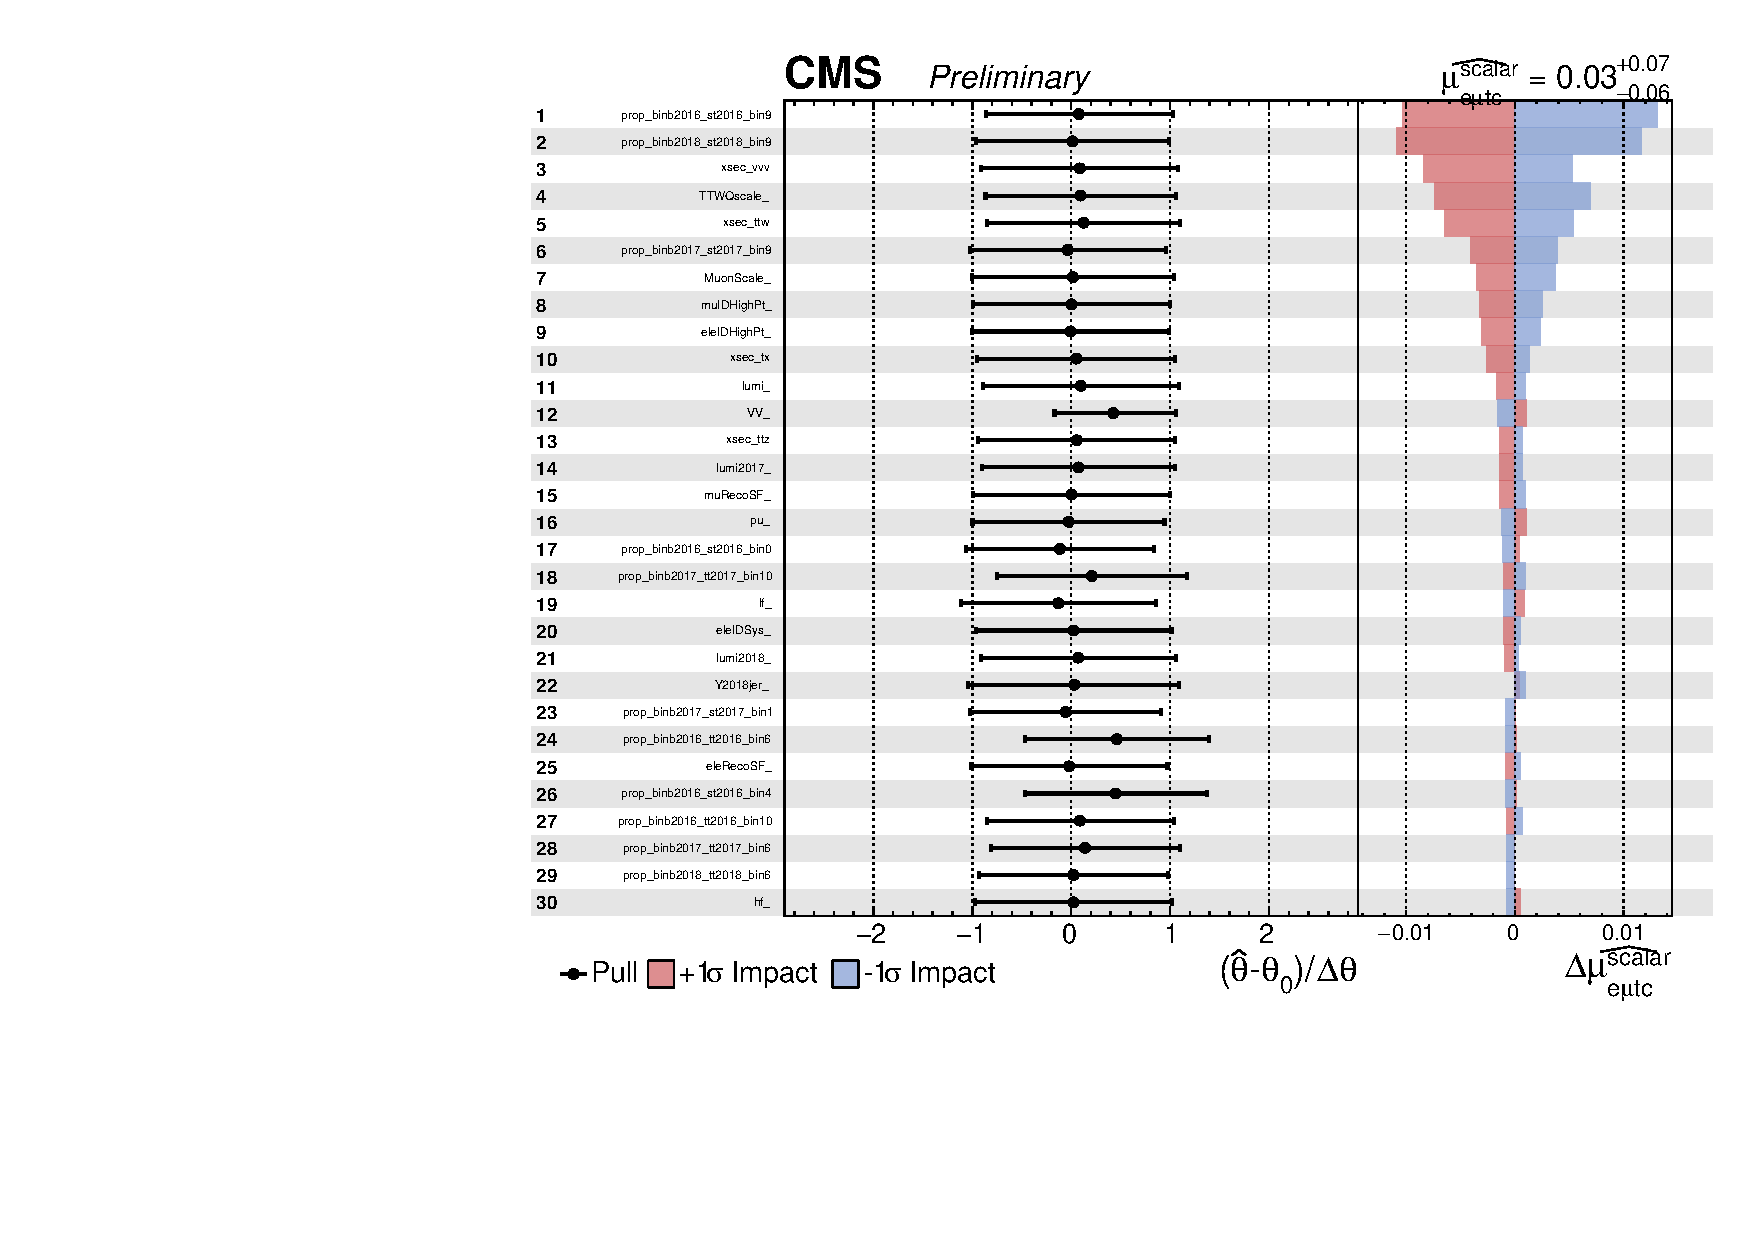
\includegraphics[width=0.48\textwidth]{figures/Appendix/Impact/Impact_ScalarC}\\
 \end{tabular}
 \caption{Impacts of nuissance parameters for run II limit setting. From top to bottom: $e\mu tc$-tensor, $e\mu tc$-vector, $e\mu tc$-scalar. From left to right: expected impact (expected signal strength at 0), observed impact.}
 \label{fig:Impact1}
 \end{center}
\end{figure}

The expected ($\mu_{exp}=$1) impacts of the nuisance parameters on the profile likelihood fit are shown in Figure \ref{fig:Impact2}.

 \begin{figure}[tbh!]
 \begin{center}
 \begin{tabular}{cc}
 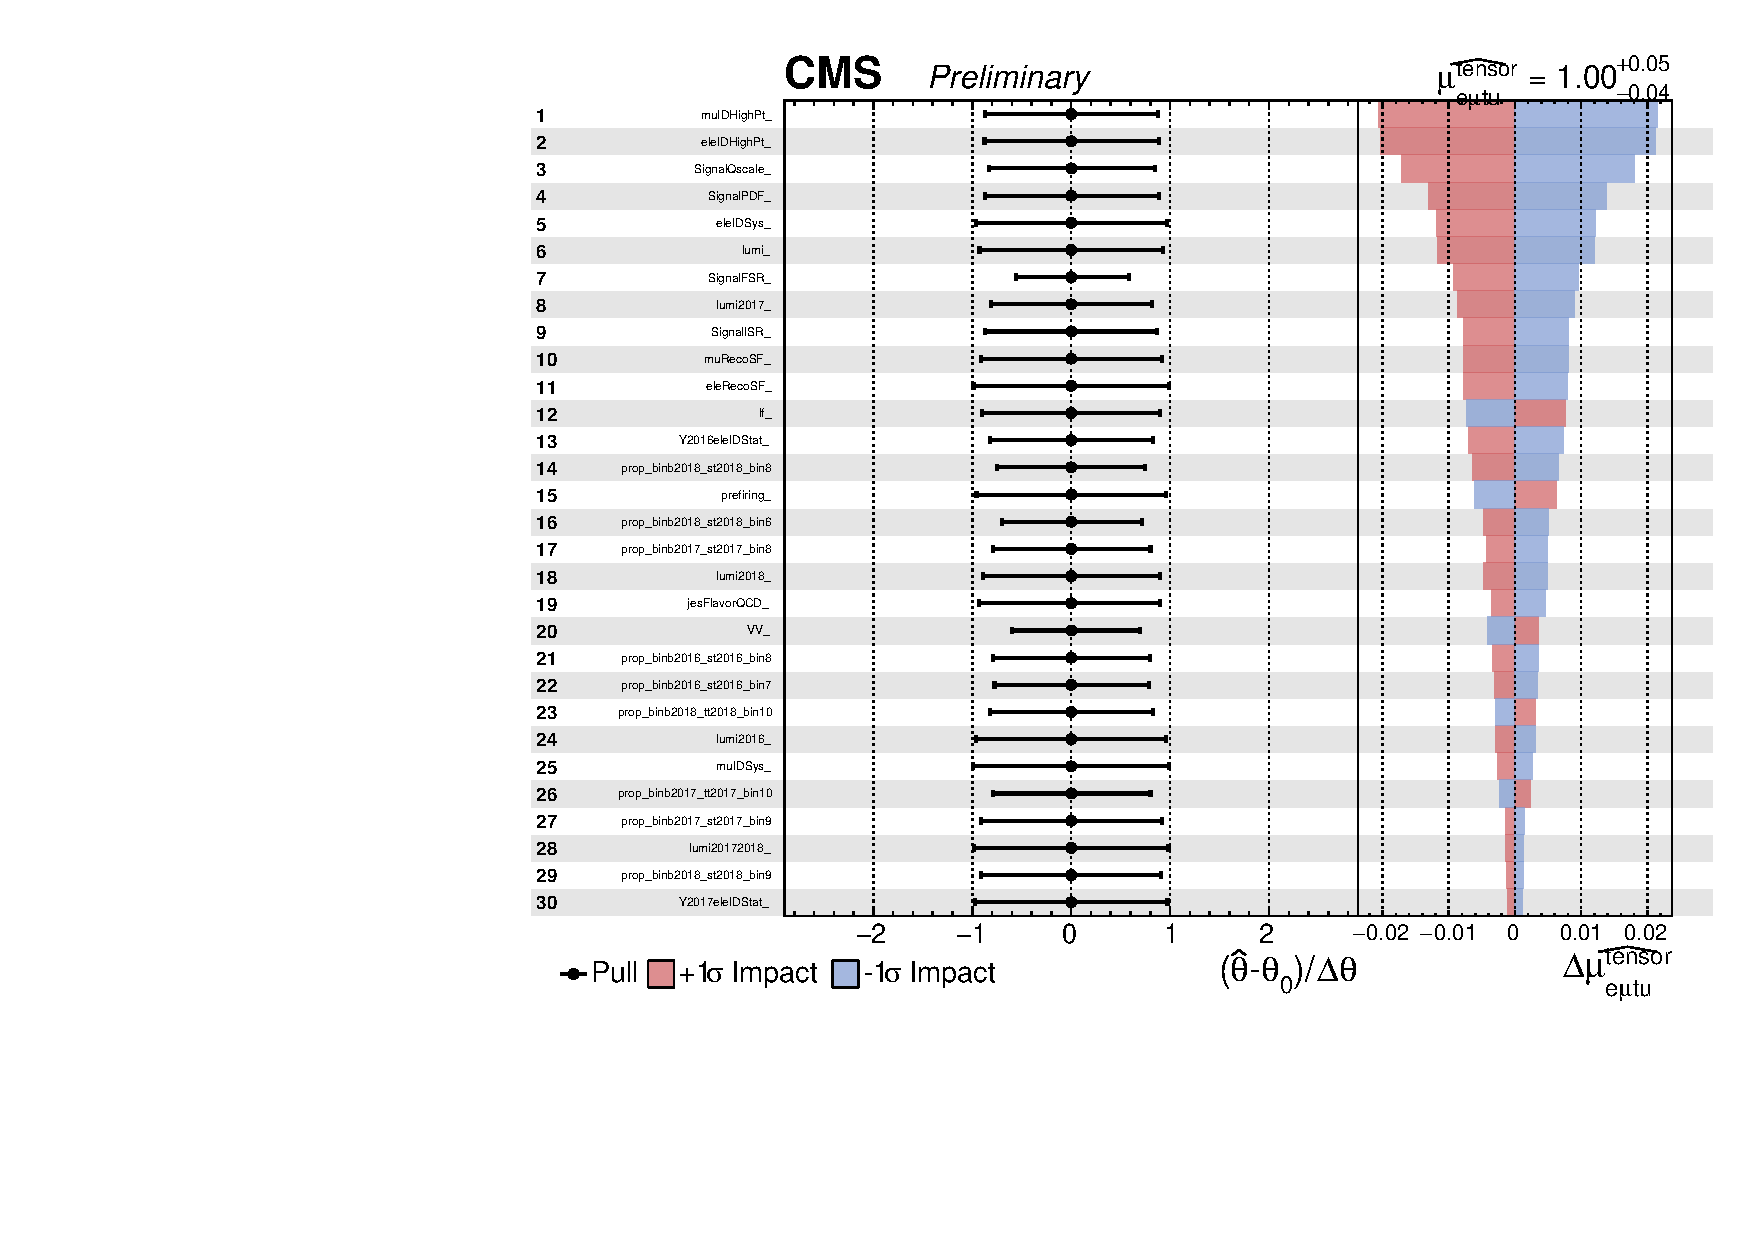
\includegraphics[width=0.48\textwidth]{figures/Appendix/Impact/Impact_TensorU_expected}&
  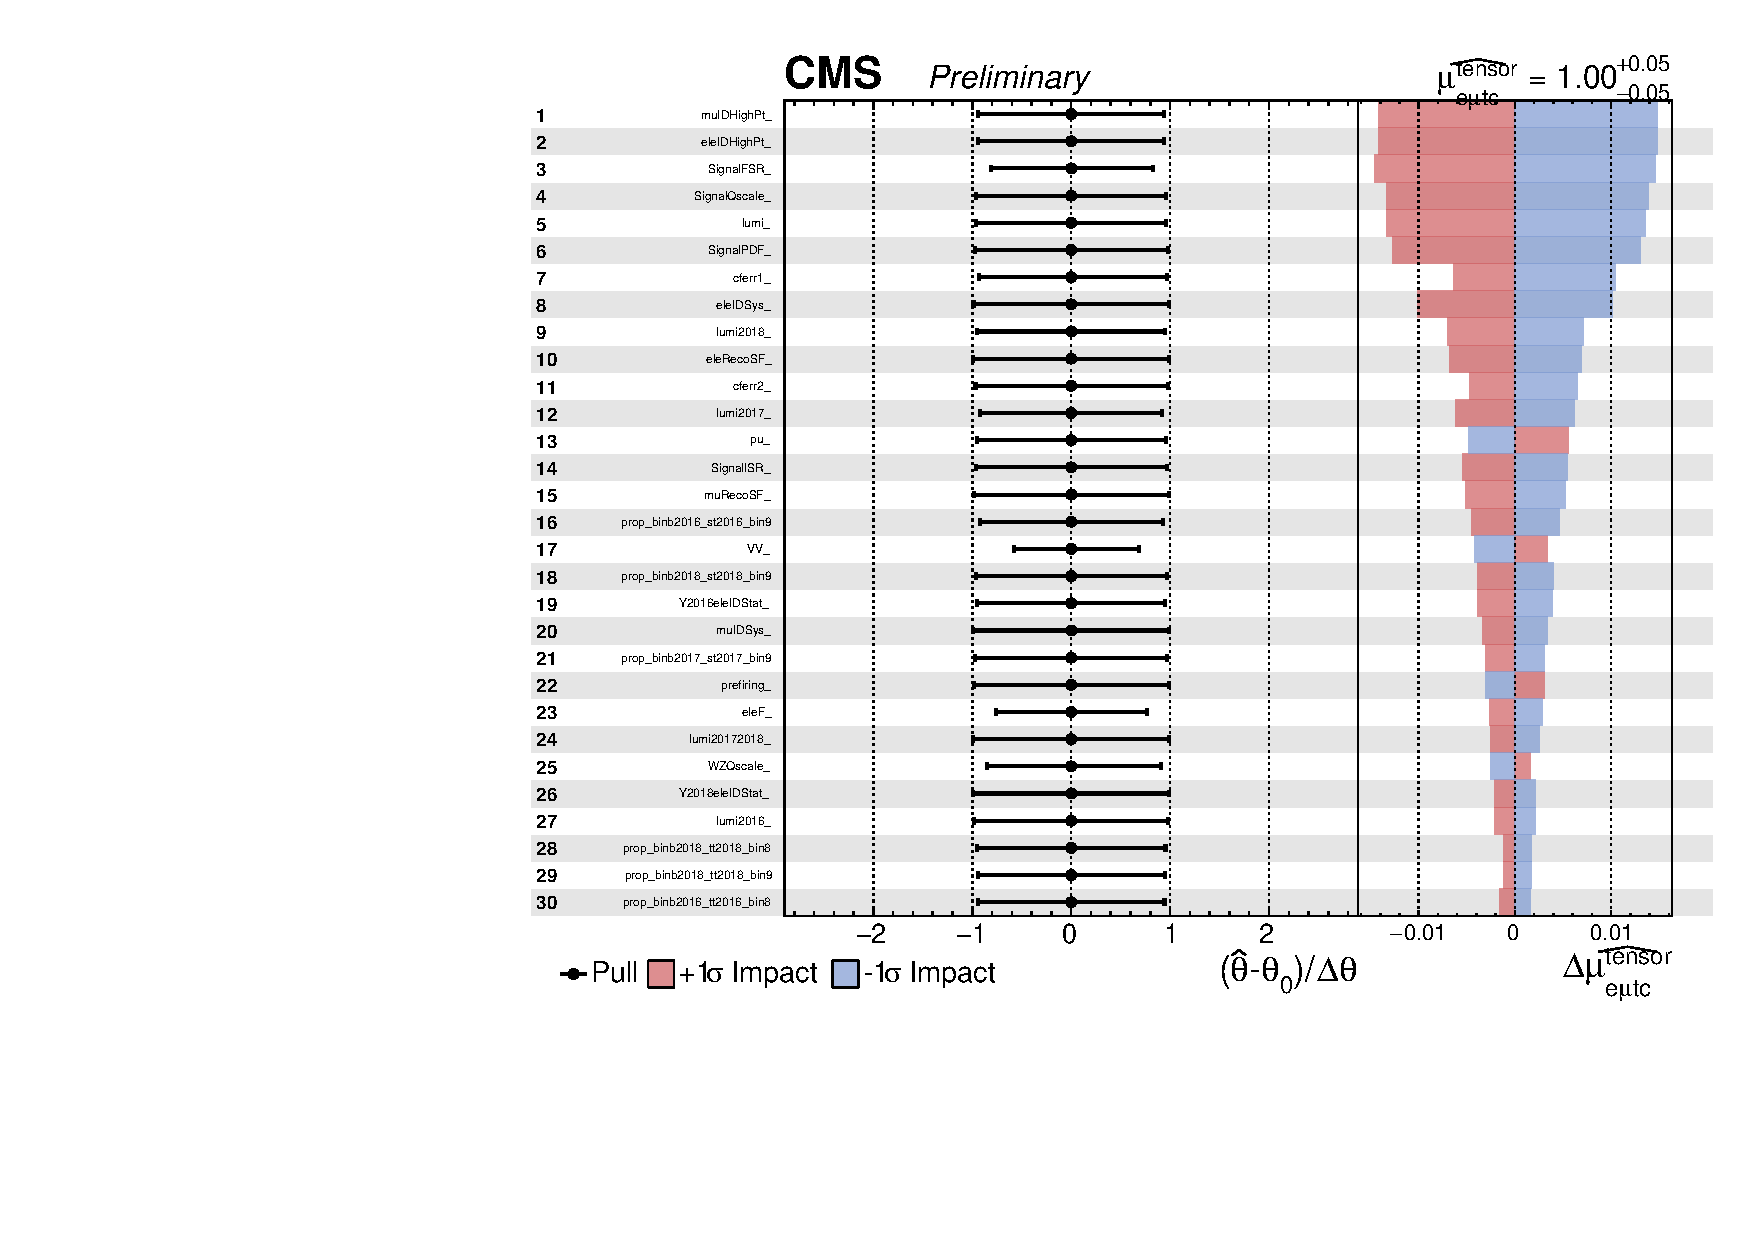
\includegraphics[width=0.48\textwidth]{figures/Appendix/Impact/Impact_TensorC_expected}\\
   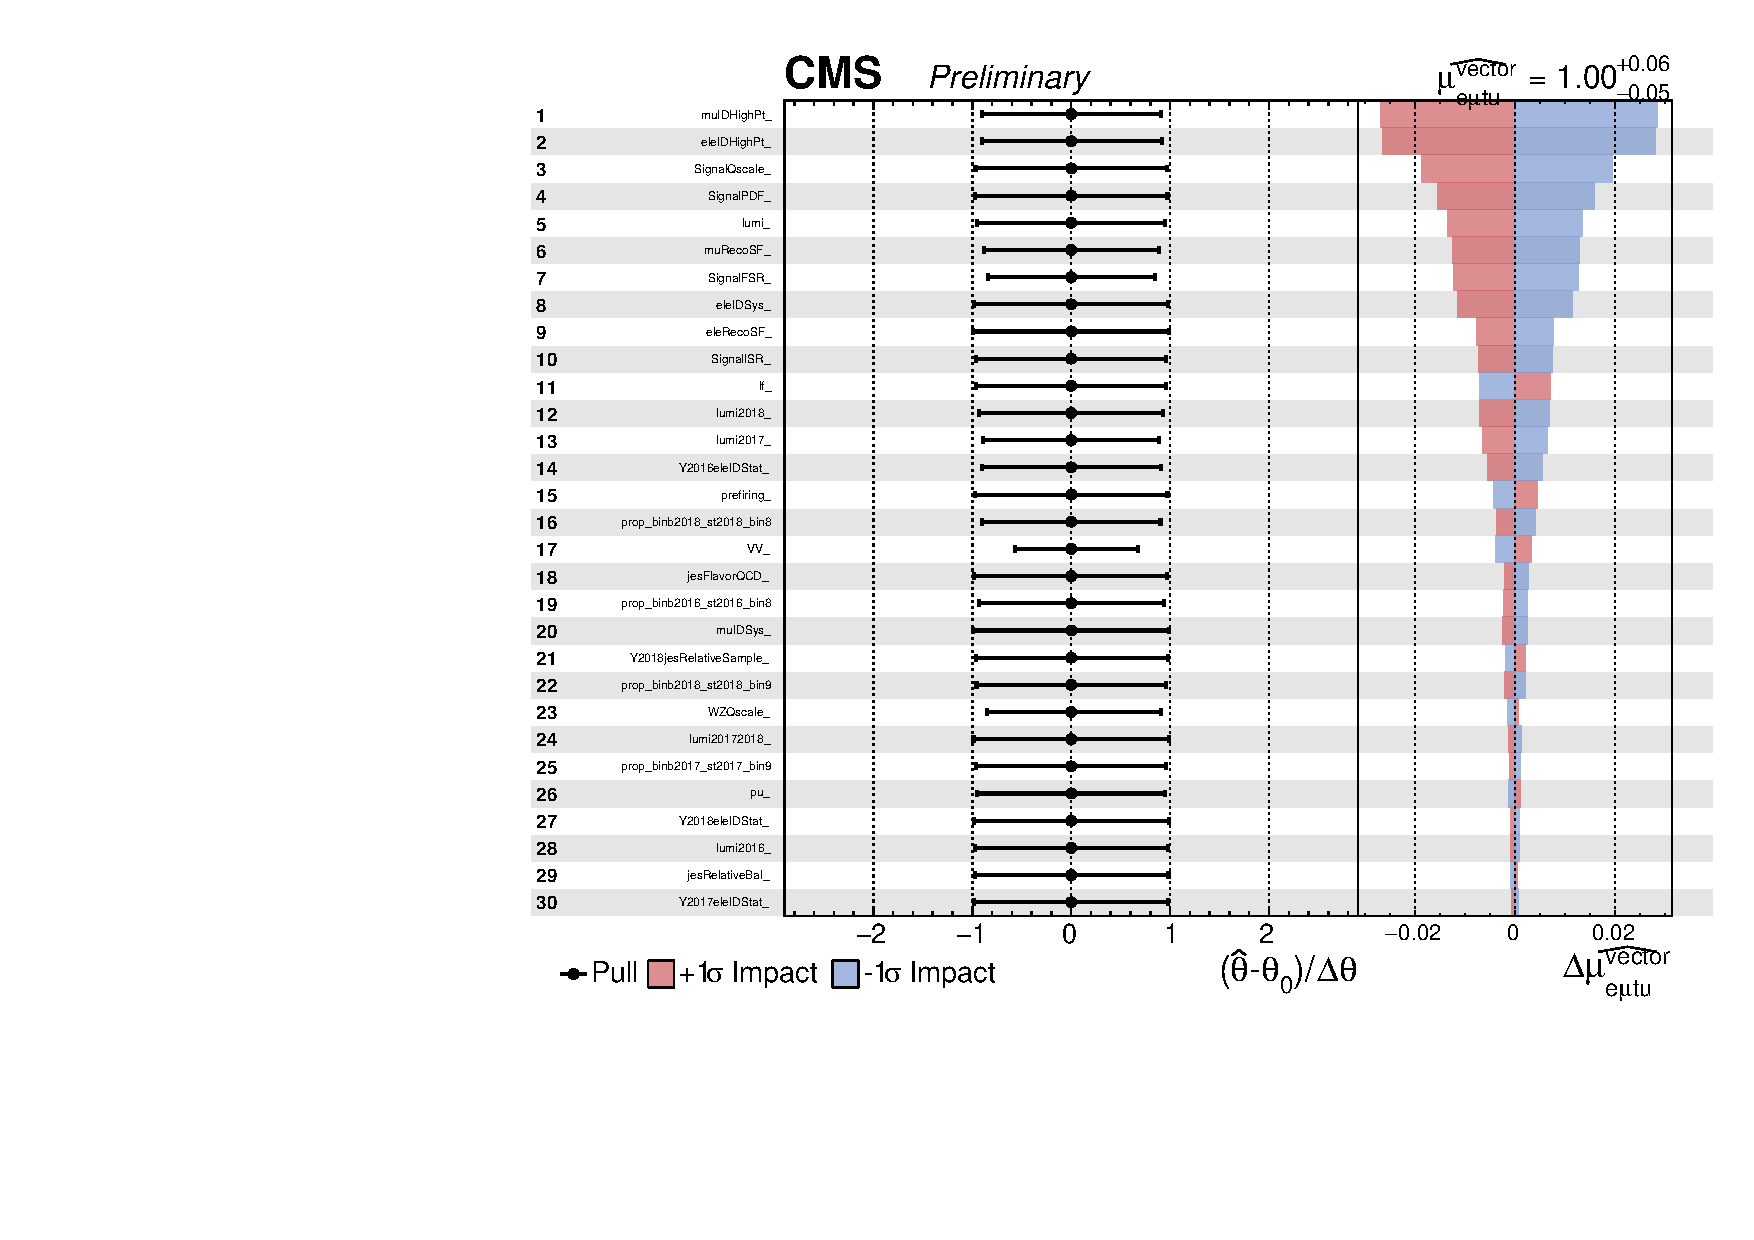
\includegraphics[width=0.48\textwidth]{figures/Appendix/Impact/Impact_VecU_expected}&
  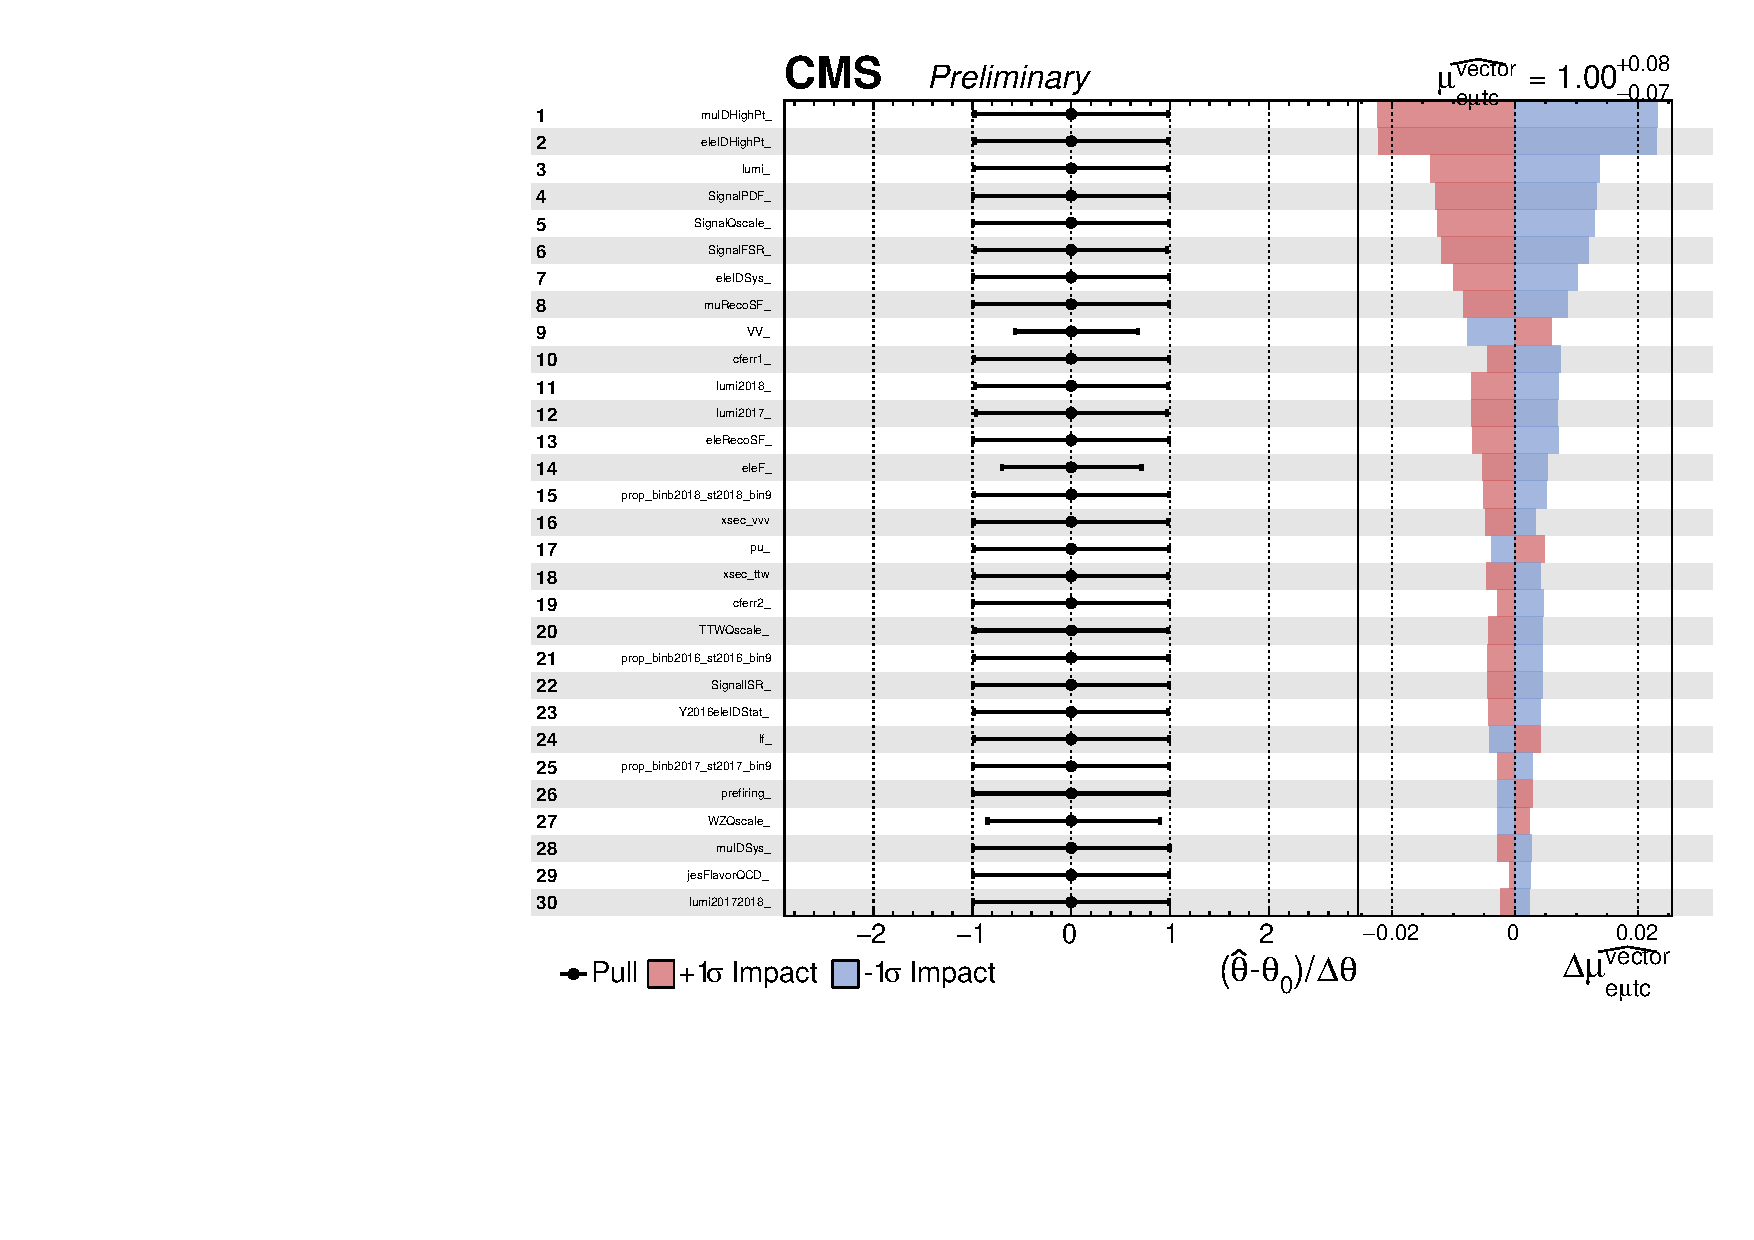
\includegraphics[width=0.48\textwidth]{figures/Appendix/Impact/Impact_VecC_expected}\\
   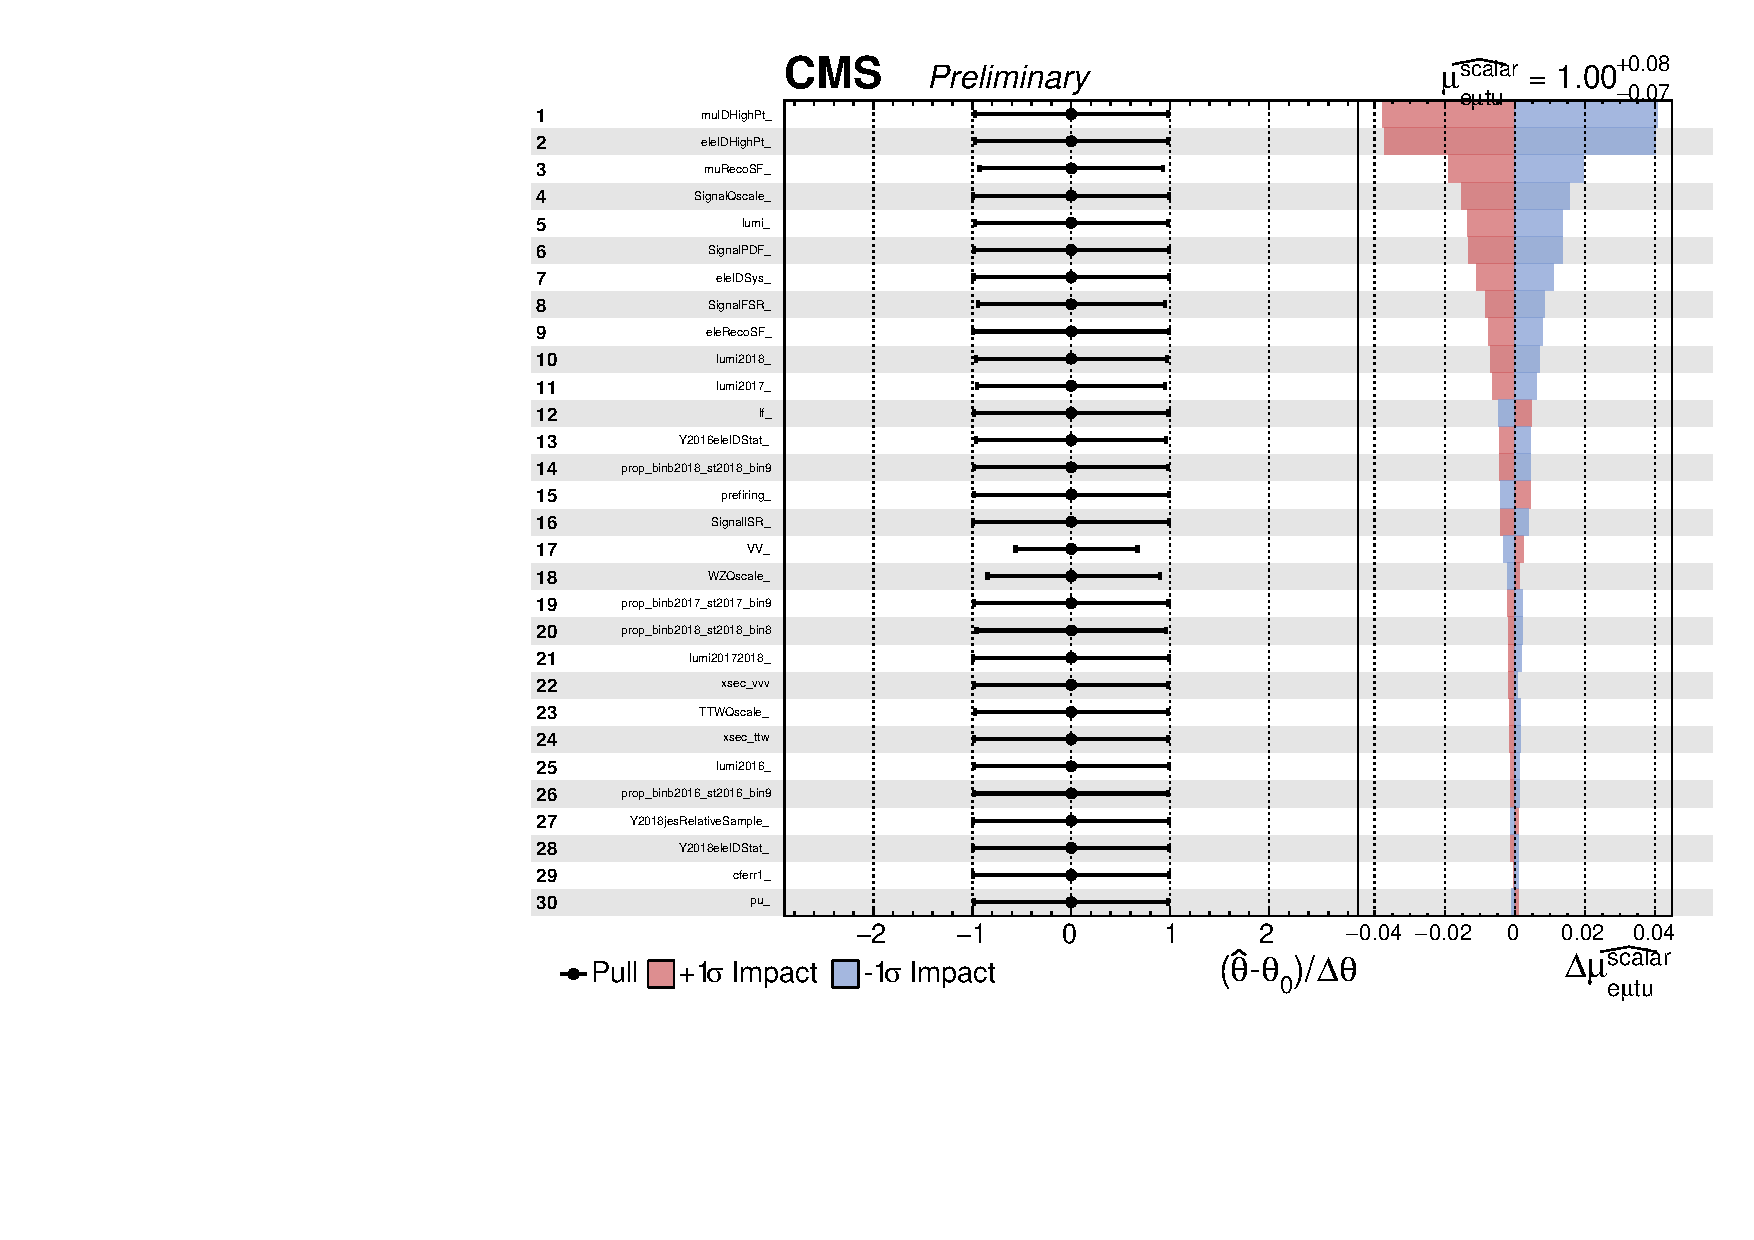
\includegraphics[width=0.48\textwidth]{figures/Appendix/Impact/Impact_ScalarU_expected}&
  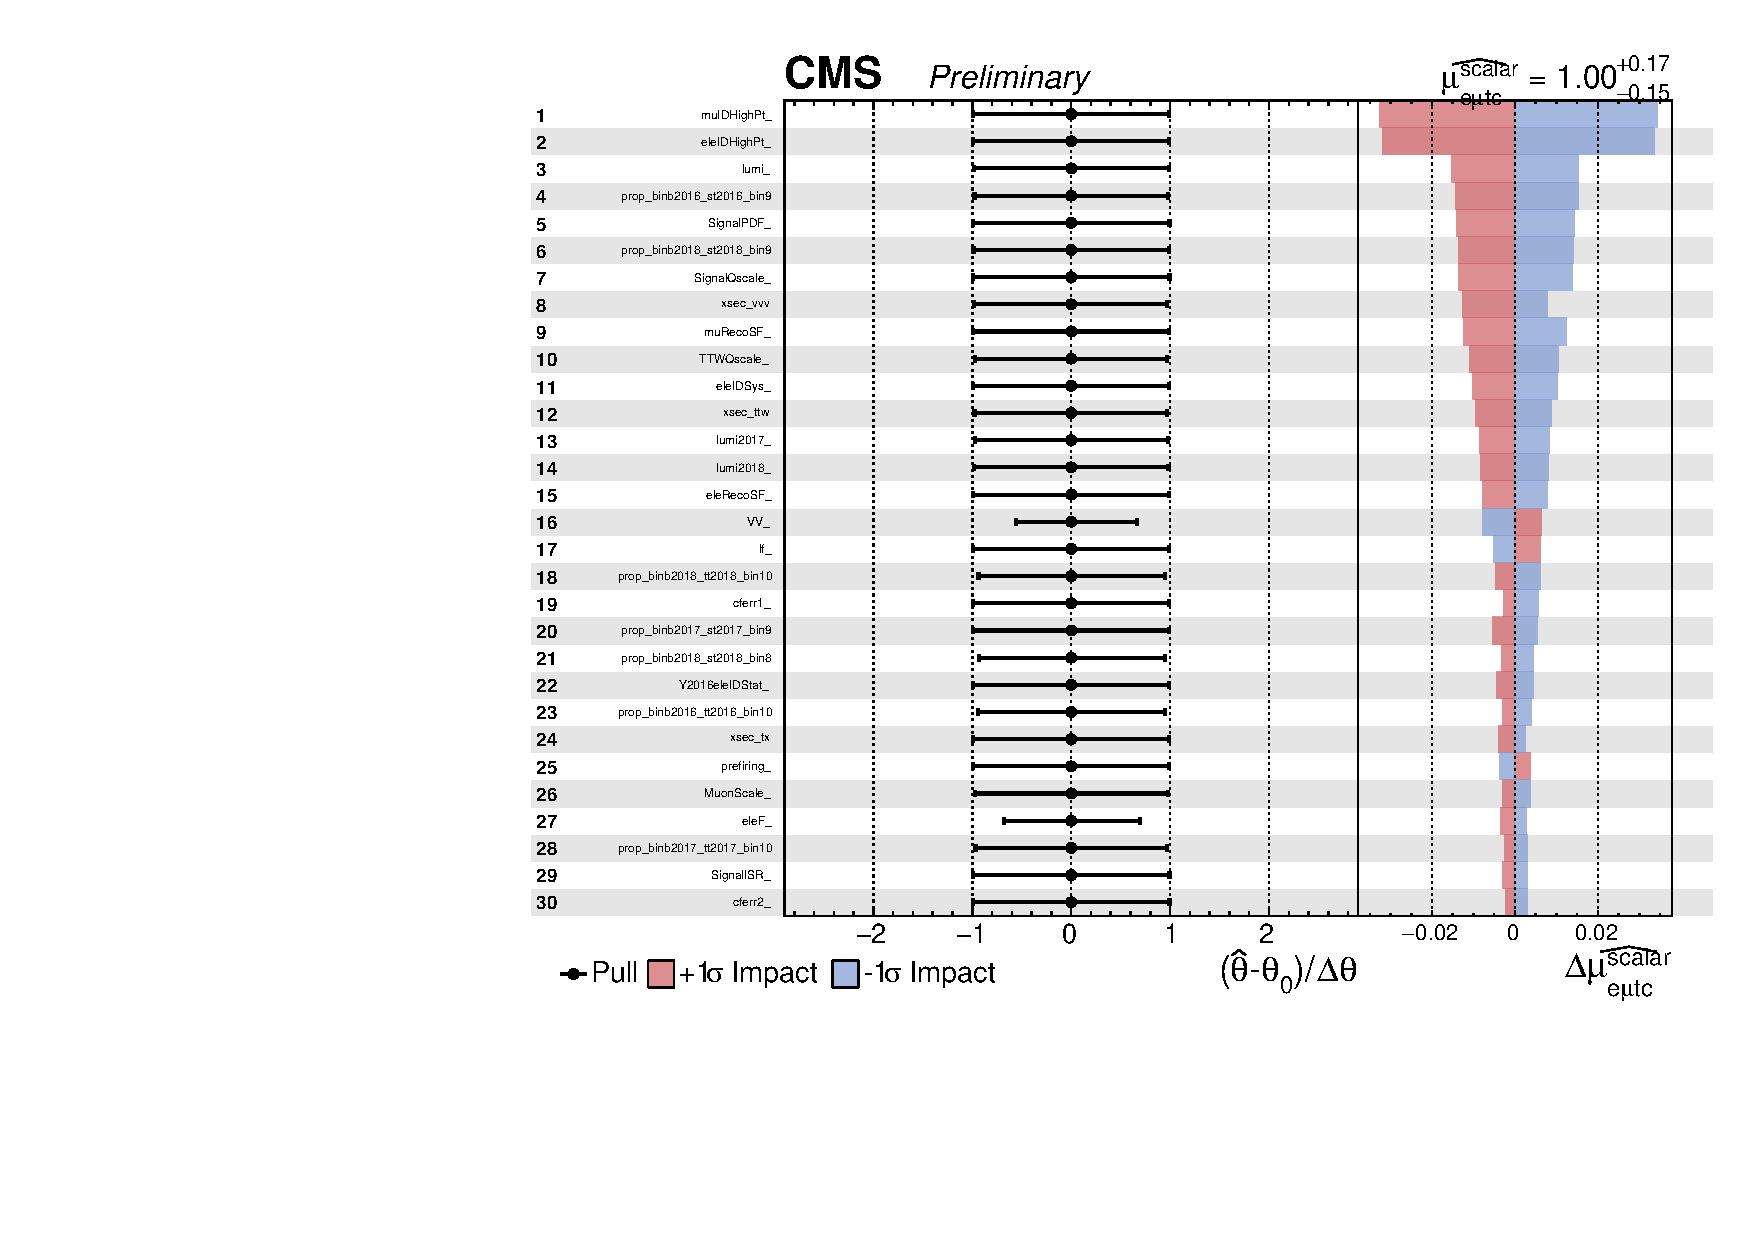
\includegraphics[width=0.48\textwidth]{figures/Appendix/Impact/Impact_ScalarC_expected}\\
 \end{tabular}
 \caption{Expected impact with an expected signal strength at 1. From top to bottom: tensor, vector, scalar. From left to right: $e\mu tu$, $e\mu tc$.}
 \label{fig:Impact2}
 \end{center}
\end{figure}
